\chapter{高阶归纳类型}
\label{cha:hits}

\index{type!higher inductive|(}%
\indexsee{inductive!type!higher}{type, higher inductive}%
\indexsee{higher inductive type}{type, higher inductive}%

\section{引言}
\label{sec:intro-hits}

\index{generation!of a type, inductive|(}

正如我们在\cref{cha:induction}中讨论的一般归纳类型那样，\emph{高阶归纳类型（higher inductive types）}也是一个用于定义由某些构造子生成新类型的一般框架。
但与普通归纳类型不同，在定义高阶归纳类型时，我们可以有一些``构造子''，它们不仅能生成该类型的\emph{点}，还能生成该类型中的\emph{道路}乃至更高维的道路。
\index{type!circle}%
\indexsee{circle type}{type,circle}%
例如，我们可以考虑由以下构造子生成的高阶归纳类型 $\Sn^1$：

\begin{itemize}
\item 一个点 $\base:\Sn^1$，以及
\item 一条道路 $\lloop : {\id[\Sn^1]\base\base}$。
\end{itemize}

这与例如 $\bool$ 的定义完全类似——$\bool$ 由
\begin{itemize}
\item 一个点 $\bfalse:\bool$ 与
\item 一个点 $\btrue:\bool$
\end{itemize}
生成，或者 $\nat$ 由
\begin{itemize}
\item 一个点 $0:\nat$ 与
\item 一个函数 $\suc:\nat\to\nat$
\end{itemize}
生成。

当我们把类型看作高阶群胚时，这种更一般的``生成''概念便十分自然：
既然高阶群胚是一种兼有点、道路和高维道路的``多排序对象''，我们就应当允许在所有维数上都有``生成元''。

我们将那些普通的构造子（例如 $\base$）称为\define{点构造子（point constructors）}
\indexdef{constructor!point}%
\indexdef{point!constructor}%
或\emph{普通构造子}，而将其他构造子（例如 $\lloop$）称为\define{道路构造子（path constructors）}
\indexdef{constructor!path}%
\indexdef{path!constructor}%
或\emph{高阶构造子}。
每个道路构造子都必须指明该道路的起点和终点，我们分别称之为其\define{源（source）}
\indexdef{source!of a path constructor}%
与\define{靶（target）}；
\indexdef{target!of a path constructor}%
对于 $\lloop$ 而言，源和靶都是 $\base$。

注意，像 $\lloop$ 这样的道路构造子会生成恒等类型中的一个\emph{新}居民，它（至少在\emph{先验}意义上）不等于任何先前已存在的此类居民。
特别地，$\lloop$ 并非\emph{先验地}等于 $\refl{\base}$（不过要证明它们确实不相等需要稍加思考，参见\cref{thm:loop-nontrivial}）。
这也正是 $\Sn^1$ 与普通归纳类型 \unit 的区别所在。

关于这一推广，有几个要点需要说明。

\index{free!generation of an inductive type}%
首先，``生成''一词应当认真对待，就如同群可以由某个集合自由生成一样。
具体来说，由于高阶群胚带有道路和高维道路上的\emph{运算}，当这样一个对象由某些构造子``生成''时，这些运算会产生更多并非直接来自构造子本身的道路。
例如，在高阶归纳类型 $\Sn^1$ 中，构造子 $\lloop$ 并不是从 $\base$ 到 $\base$ 的唯一非平凡道路；
我们还有``$\lloop\ct\lloop$''、``$\lloop\ct\lloop\ct\lloop$''等等，以及 $\opp{\lloop}$ 等，它们全都各不相同。
这可能看起来显而易见，甚至不值一提，但它偏离了``普通''归纳类型的行为：
在普通归纳类型中，除了构造子直接``放入''的内容之外，不应期待看到其他东西。

其次，这种生成实际上是\emph{自由}生成：高阶归纳类型严格来说并不允许我们施加``公理''，例如强行要求``$\lloop\ct\lloop$''等于 $\refl{\base}$。
然而，在 $\infty$-群胚的世界里，%
\index{.infinity-groupoid@$\infty$-groupoid}
``自由生成''与``展示''之间几乎没有差别，
\index{presentation!of an infinity-groupoid@of an $\infty$-groupoid}%
\index{generation!of an infinity-groupoid@of an $\infty$-groupoid}%
因为我们可以通过添加一个新的二维生成元（例如在 $\base=\base$ 中添加一条道路 $\lloop\ct\lloop = \refl{\base}$）来使两条道路\emph{在同伦意义下}相等。
当然，我们随后还需要考虑这个新生成元是否应当满足它自己的``公理''，依此类推；但原则上，任何``展示''都可以通过将公理转化为构造子来变成``自由''生成。
正如我们将要看到的，通过添加``截断构造子''，我们同样可以用高阶归纳类型来表达诸如群展示之类的经典概念。

第三，尽管高阶归纳类型包含了能在该类型中生成\emph{道路}的“构造子”，它仍然是对\emph{单个}类型的归纳定义。
特别地，正如我们将要看到的，具有泛性质（通常由归纳原理表述）的是高阶归纳类型本身，而\emph{不是}它的相等类型。
高阶归纳类型的相等类型保留了所有相等类型通常的归纳原理（即道路归纳），并不会获得任何新的归纳原理。

因此，以具体方式确定高阶归纳类型的相等类型可能并非易事；这与\cref{cha:basics}中的情况不同，在那里我们能够对所有传统类型形成操作下相等类型的行为给出明确描述。
例如，在 $\Sn^1$ 中，是否存在从 $\base$ 到 $\base$ 的道路，它不仅仅是 $\lloop$ 及其逆的复合？
直觉上答案似乎是否定的（事实上确实如此），但证明这一点绝非易事。
实际上，这类问题迅速将我们引向诸如计算球面同伦群这样的难题——这是代数拓扑中长期悬而未决的问题，目前尚未知简单的公式。
同伦类型论为这类问题带来了强大的新视角，但也要求类型论本身变得与这些问题的答案一样复杂。

\index{dimension!of path constructors}%
第四，构造子的“维度”（即它们输出的是点、道路、道路之间的道路等等）与结果类型在哪些维度具有非平凡同伦没有直接联系。
举个简单的例子：如果归纳类型 $B$ 有一个类型为 $A\to B$ 的构造子，那么 $A$ 中的任何道路和高阶道路都会在 $B$ 中产生相应的道路和高阶道路，即使该构造子根本不是“高阶”构造子。
对于高阶构造子同样如此：具有一个类型为 $A\to (\id[B]xy)$ 的构造子，不仅意味着 $A$ 中的点会在 $B$ 中生成从 $x$ 到 $y$ 的道路，还意味着 $A$ 中的道路会生成这些道路之间的道路，依此类推。
我们将看到，这种可能性正是高阶归纳类型如此强大的主要原因。

另一方面，即便构造子的输入中\emph{没有}高阶类型，也有可能生成“意想不到的”高阶道路。
例如，在由以下构造生成的二维球面 $\Sn^2$ 中：
\symlabel{s2a}
\index{type!2-sphere}%

\begin{itemize}
\item 一个点 $\base:\Sn^2$，以及
\item 一条在 ${\base=\base}$ 中的 2-维道路$\surf:\refl{\base} = \refl{\base}$，
\end{itemize}

存在一条从 $\refl{\refl{\base}}$ 到自身的非平凡\emph{3-维道路}。
拓扑学家会认出这条道路是\emph{Hopf 纤维化}的一种体现。
从范畴论的观点来看，这与前文提到的 $\Sn^1$ 不仅包含 $\lloop$ 还包含 $\lloop\ct\lloop$ 等现象属于同类：只不过在\emph{高阶}群胚中，存在能够提升维度的\emph{运算}。
事实上，我们在\cref{sec:equality}中已经见过许多这类运算：结合律和单位律不仅仅是性质，还是运算——它们的输入是 1-道路，输出是 2-道路。

\index{generation!of a type, inductive|)}%

% In US Trade format it wants a page break here but then it stretches the above itemize,
% so we give it some stretchable space to use if it wants to.
\vspace*{0pt plus 20ex}

\section{归纳原理与依值道路}
\label{sec:dependent-paths}

当我们描述诸如圆周这样的高阶归纳类型是由某些构造子生成时，必须通过给出类似于\cref{cha:typetheory}中基本类型构造子的规则来解释这意味着什么。
构造子本身给出了\emph{引入（introduction）}规则，但要解释\emph{消去（elimination）}规则（即归纳原理和递归原理），则需要多费些思量。
在本书中，我们不打算给出一个一般性的形式化表述，来界定什么算作“高阶归纳定义”以及如何从这样的定义中提取消去规则——事实上，这是一个微妙的问题，也是当前研究的课题。
相反，我们将依赖一些一般性的非正式讨论和大量例子。

\index{type!circle}%
\index{recursion principle!for S1@for $\Sn^1$}%
递归原理通常比较容易描述：给定一个类型，只要它配备了与所讨论的高阶归纳类型的构造子所赋予的相同结构，就存在一个将构造子映射到该结构的函数。
例如，就 $\Sn^1$ 而言，其递归原理说的是：给定任意配备了基点 $b:B$ 和道路 $\ell:b=b$ 的类型 $B$，存在一个函数 $f:\Sn^1\to B$，使得 $f(\base)=b$ 且 $\apfunc f (\lloop) = \ell$。

\index{computation rule!for S1@for $\Sn^1$}%
\index{equality!definitional}%
后两个等式就是\emph{计算规则}。
\index{computation rule!for higher inductive types|(}%
\index{computation rule!propositional|(}%
然而，这里存在一个问题：这些计算规则应该是\index{judgmental equality}判断相等性还是命题相等性（道路）？
对于普通的归纳类型，我们曾毫不犹豫地将其设为判断相等性，尽管我们在\cref{cha:induction}中看到，即使将其设为命题相等性，在等价的意义下仍会得到相同的类型。
在普通情形下，可以论证计算规则在引言所描述的直观意义下确实是\emph{定义性}相等。

\index{equality!judgmental}%
但对于高阶归纳类型，这一点就不那么清晰了。%, and it is likewise less clear to what extent these equalities can be made judgmental in the known set-theoretic models.
此外，由于操作 $\apfunc f$ 并非类型论真正的基本组成部分，而是我们利用相等类型的归纳原理\emph{定义}出来的（而且我们本可选择其他等价的方式来定义），在一条\emph{判断}相等性中显式地引用它似乎并不合适。
判断相等性是演绎系统的一部分，而演绎系统不应该依赖于我们可能在该系统\emph{内部}做出的特定定义选择。
同时还需要考虑语义和实现方面的问题；详见注记。

不过，将高阶归纳类型的\emph{点}构造子的计算规则设为判断相等性，似乎是没有问题的。
在上面的例子中，这就意味着我们有 $f(\base)\jdeq b$。
这一选择有利于从计算的角度理解高阶归纳类型。
同时，它也极大地简化了我们的工作，因为否则第二个计算规则 $\apfunc f (\lloop) = \ell$ 甚至无法作为命题相等性而良类型；我们将不得不在等式的一边或另一边复合上 $f(\base)$ 与 $b$ 之间指定的那个相等证明。
（当然，当我们讨论更高维的道路时，这类问题最终确实会出现，但在此我们无需对此过于担忧。
亦可参见\cref{sec:hubs-spokes}。）
因此，我们将点构造子的计算规则取为判断相等性，而将道路以及更高维道路的计算规则取为命题相等性。%
\footnote{特别地，用\cref{sec:types-vs-sets}的语言来说，这意味着我们的高阶归纳类型是一种混合体：既有\emph{规则}（规定如何引入此类类型及其元素、其归纳原理、以及其点构造子的计算规则），也有\emph{公理}（道路构造子的计算规则，它们断言某些相等类型\index{inhabited}有实例，且给出实例的项未另行指定）。
我们可以期望，将来能够出现一种更好的类型理论，在其中，高阶归纳类型——就像泛等性一样——将仅通过规则而不借助公理来呈现。%
\indexfoot{axiom!versus rules}%
\indexfoot{rule!versus axioms}%
}

\begin{rmk}\label{rmk:defid}
回忆一下，对于普通的归纳类型，我们将递归定义的函数的计算规则不仅视为判断相等性，而且视作\emph{定义性}相等，因此可以使用符号 $\defeq$ 来表示它们。
例如，截断的前驱\index{predecessor!function, truncated}函数 $p:\nat\to\nat$ 就是由 $p(0)\defeq 0$ 和 $p(\suc(n))\defeq n$ 定义的。
对于高阶归纳类型，这类记号对点构造子是合理的（例如 $f(\base)\defeq b$），但对于道路构造子则可能产生误导，因为像 $\ap f \lloop = \ell$ 这样的相等性并非判断相等性。
因此，我们混合使用记法，将这种``通过定义的命题相等性''写作 $\ap f \lloop \defid \ell$。
\end{rmk}


\index{computation rule!for higher inductive types|)}%
\index{computation rule!propositional|)}%

\index{type!circle|(}%
\index{induction principle!for S1@for $\Sn^1$}%
那么，归纳原理（依值消去子）又是怎样的呢？
回想一下，对于一个普通的归纳类型 $W$，为了用归纳法证明 $\prd{x:W} P(x)$，我们必须为 $W$ 的每个构造子指定一个 $P$ 上的操作，该操作作用于 $W$ 中该构造子``上方''的``纤维''上。
例如，如果 $W$ 是自然数 $\nat$，那么要归纳地证明 $\prd{x:\nat} P(x)$，我们必须指定


\begin{itemize}
\item 一个位于构造子 $0:\nat$ 上方纤维中的元素 $b:P(0)$，以及
\item 对于每个 $n:\nat$，一个函数 $P(n) \to P(\suc(n))$。
\end{itemize}


第二个条件可以看作一个位于构造子 $\suc:\nat\to\nat$ \emph{上方}的``$P\to P$''函数，这推广了 $b:P(0)$ 位于构造子 $0:\nat$ 上方的方式。

因此，类比之下，为了证明 $\prd{x:\Sn^1} P(x)$，我们应当指定

\begin{itemize}
\item 在构造子 $\base:\Sn^1$ 上方纤维中的一个元素 $b:P(\base)$，以及
\item 一条从 $b$ 到 $b$、``落在构造子 $\lloop:\base=\base$ 上方''的道路。
\end{itemize}

注意，尽管 $\Sn^1$ 还包含 $\lloop$ 以外的其他道路（例如 $\refl{\base}$ 和 $\lloop\ct\lloop$），我们只需指定一条落在构造子\emph{本身}上方的道路。
这表达了 $\Sn^1$ 由其构造子``自由生成''的直观。

然而，问题在于一条道路``落在''另一条道路``上方''究竟是什么意思。
它当然\emph{不}意味着仅仅是一条 $b=b$ 的道路，因为那将是纤维 $P(\base)$ 中的道路（从拓扑上说，是一条落在 $\base$ 处\emph{常值}道路上方的道路）。
不过，实际上我们已经在\cref{cha:basics}中回答了这个问题：在\cref{lem:mapdep}之前的讨论中，我们得出结论，一条从 $u:P(x)$ 到 $v:P(y)$ 且落在 $p:x=y$ 上方的道路，可以表示为纤维 $P(y)$ 中的道路 $\trans p u = v$。
由于本章将大量使用这样的\define{依值道路}
\index{path!dependent}%
，我们为此引入一个专门的记号：
\begin{equation}
  (\dpath P p u v) \defeq (\transfib{P} p u = v).\label{eq:dpath}
\end{equation}

\begin{rmk}
定义依值道路还有其他可能的方式。
例如，除了 $\trans p u = v$，我们也可以考虑$u = \trans{(\opp p)}{v}$。
我们还可以将其视为更一般的``异质相等''的特例，
\index{heterogeneous equality}%
\index{equality!heterogeneous}%
或者直接定义为一个归纳类型族。
所有这些定义都给出等价的类型，因此在这个意义上选择哪一个并不太重要。
然而，选择 $\trans p u = v$ 作为定义，使我们最容易推导出关于依值道路的其他结论，例如 $\apdfunc{f}$ 会给出这样的道路，或者我们可以利用\cref{sec:computational}中的传输引理在特定的类型族中计算它们。
\end{rmk}

有了依值道路的概念，我们现在可以更精确地表述 $\Sn^1$ 的归纳原理：给定 $P:\Sn^1\to\type$ 以及
\begin{itemize}
\item 一个元素 $b:P(\base)$，和
\item 一条道路 $\ell : \dpath P \lloop b b$，
\end{itemize}
则存在一个函数$f:\prd{x:\Sn^1} P(x)$，满足 $f(\base)\jdeq b$ 且 $\apd f \lloop = \ell$。
与非依值的情形一样，我们说通过 $f(\base)\defeq b$ 与 $\apd f \lloop \defid \ell$ 来定义 $f$。

\begin{rmk}\label{rmk:varies-along}
在非正式地描述这一归纳原理的某个应用时，我们将其视为把目标``对所有 $x:\Sn^1$ 有 $P(x)$''拆分为两种情形，并有时分别以``当 $x$ 是 $\base$ 时''和``当 $x$ 沿 $\lloop$ 变化时''这样的说法来引入。
``沿一条道路变化''并没有特定的数学含义：它只是一种方便的说法，用以指示证明中相应部分的开始；参见\cref{thm:S1-autohtpy}中的例子。
\index{vary along a path constructor}%
\end{rmk}

从拓扑上说，$\Sn^1$ 的归纳原理可以如\cref{fig:topS1ind}所示来可视化。给定圆上的一个纤维化（图中是环面），定义该纤维化的一个截面，就等同于给出基点 $\base$ 上方纤维中的一个点 $b$，以及一条落在 $\lloop$ 上方、从 $b$ 到 $b$ 的道路。按照我们对依值道路的定义，这一点的类型论解释如\cref{fig:ttS1ind}所示：落在 $\lloop$ 上方、从 $b$ 到 $b$ 的道路，由基点上方纤维中从 $\trans \lloop b$ 到 $b$ 的道路来表示。

\begin{figure}
  \centering
  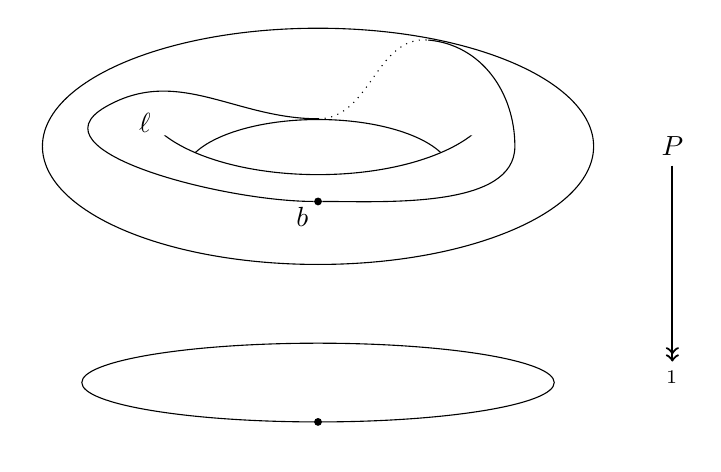
\begin{tikzpicture}
    \draw (0,0) ellipse (3 and .5);
    \draw (0,3) ellipse (3.5 and 1.5);
    \begin{scope}[yshift=4]
      \clip (-3,3) -- (-1.8,3) -- (-1.8,3.7) -- (1.8,3.7) -- (1.8,3) -- (3,3) -- (3,0) -- (-3,0) -- cycle;
      \draw[clip] (0,3.5) ellipse (2.25 and 1);
      \draw (0,2.5) ellipse (1.7 and .7);
    \end{scope}
    \node (P) at (4.5,3) {$P$};
    \node (S1) at (4.5,0) {$\Sn^1$};
    \draw[->>,thick] (P) -- (S1);
    \node[fill,circle,inner sep=1pt,label={below right:$\base$}] at (0,-.5) {};
    \node at (-2.6,.6) {$\lloop$};
    \node[fill,circle,\OPTblue,inner sep=1pt] (b) at (0,2.3) {};
    \node[\OPTblue] at (-.2,2.1) {$b$};
      \begin{scope}
        \draw[\OPTblue] (b) to[out=180,in=-150] (-2.7,3.5) to[out=30,in=180] (0,3.35);
        \draw[\OPTblue,dotted] (0,3.35) to[out=0,in=175] (1.4,4.35);
        \draw[\OPTblue] (1.4,4.35) to[out=-5,in=90] (2.5,3) to[out=-90,in=0,looseness=.8] (b);
      \end{scope}
      \node[\OPTblue] at (-2.2, 3.3) {$\ell$};
  \end{tikzpicture}
  \caption{$\Sn^1$ 的拓扑归纳原理}
  \label{fig:topS1ind}
\end{figure}

\begin{figure}
  \centering
  \begin{tikzpicture}
    \draw (0,0) ellipse (3 and .5);
    \draw (0,3) ellipse (3.5 and 1.5);
    \begin{scope}[yshift=4]
      \clip (-3,3) -- (-1.8,3) -- (-1.8,3.7) -- (1.8,3.7) -- (1.8,3) -- (3,3) -- (3,0) -- (-3,0) -- cycle;
      \draw[clip] (0,3.5) ellipse (2.25 and 1);
      \draw (0,2.5) ellipse (1.7 and .7);
    \end{scope}
    \node (P) at (4.5,3) {$P$};
    \node (S1) at (4.5,0) {$\Sn^1$};
    \draw[->>,thick] (P) -- (S1);
    \node[fill,circle,inner sep=1pt,label={below right:$\base$}] at (0,-.5) {};
    \node at (-2.6,.6) {$\lloop$};
    \node[fill,circle,\OPTblue,inner sep=1pt] (b) at (0,2.3) {};
      \node[\OPTblue] at (-.3,2.3) {$b$};
      \node[fill,circle,\OPTpurple,inner sep=1pt] (tb) at (0,1.8) {};
      % \draw[\OPTpurple,dashed] (b) to[out=0,in=0,looseness=5] (0,4) to[out=180,in=180] (tb);
      \draw[\OPTpurple,dashed] (b) arc (-90:90:2.9 and 0.85) arc (90:270:2.8 and 1.1);
      \begin{scope}
        \clip (b) -- ++(.1,0) -- (.1,1.8) -- ++(-.2,0) -- ++(0,-1) -- ++(3,2) -- ++(-3,0) -- (-.1,2.3) -- cycle;
        \draw[\OPTred,dotted,thick] (.2,2.07) ellipse (.2 and .57);
        \begin{scope}
          % \draw[clip] (b) -- ++(.1,0) |- (tb) -- ++(-.2,0) -- ++(0,-1) -| ++(3,3) -| (b);
          \clip (.2,0) rectangle (-2,3);
          \draw[\OPTred,thick] (.2,2.07) ellipse (.2 and .57);
        \end{scope}
      \end{scope}
      \node[\OPTred] at (1,1.2) {$\ell: \trans \lloop b=b$};
  \end{tikzpicture}
  \caption{$\Sn^1$ 的类型论归纳原理}
  \label{fig:ttS1ind}
\end{figure}

当然，我们期望能够从归纳原理推导出递归原理，只需取 $P$ 为一个常值类型族即可。
事实上确实如此，不过，从关于 $\lloop$ 的依值计算规则（涉及 $\apdfunc f$）推导出其非依值的版本（涉及 $\apfunc f$），这一步比预想的要棘手一些。

\begin{lem}\label{thm:S1rec}
  \index{recursion principle!for S1@for $\Sn^1$}%
  \index{computation rule!for S1@for $\Sn^1$}%
  若 $A$ 是一个类型，且给定 $a:A$ 与 $p:\id[A]aa$，则存在函数 $f:\Sn^1\to{}A$ 满足
  \begin{align*}
    f(\base)&\defeq a \\
    \apfunc f(\lloop)&\defid p.
  \end{align*}
\end{lem}

\begin{proof}
  我们希望将 $\Sn^1$ 的归纳原理应用于常值类型族，即 $(\lam{x} A): \Sn^1\to \UU$。
  为此所需的前提是：$(\lam{x} A)(\base) \jdeq A$ 中的一个点（即 $a:A$），以及一条 $\dpath {x \mapsto A}{\lloop} a a$ 中的依值道路（或等价地说，$\transfib{x \mapsto A}{\lloop} a = a$）。
  后一个类型并非 $p$ 所在的类型 $\id[A]aa$，但它与后者等价，因为根据 \cref{thm:trans-trivial}，我们有 $\transconst{A}{\lloop}{a} : \transfib{x \mapsto A}{\lloop} a= a$。
  因此，给定 $a:A$ 与 $p:a=a$，我们可以考虑复合道路
  \[\transconst{A}{\lloop}{a} \ct p:(\dpath {x \mapsto A}\lloop aa).\]
  应用归纳原理，我们得到 $f:\Sn^1\to A$，使得
  \begin{align}
    f(\base) &\jdeq a \qquad\text{and}\label{eq:S1recindbase}\\
    \apdfunc f(\lloop) &= \transconst{A}{\lloop}{a} \ct p.\label{eq:S1recindloop}
  \end{align}
  接下来需要推导等式 $\apfunc f(\lloop)=p$。
  然而，根据 \cref{thm:apd-const}，我们有
  \[\apdfunc f(\lloop) = \transconst{A}{\lloop}{f(\base)} \ct \apfunc f(\lloop).\]
  将此式与 \eqref{eq:S1recindloop} 结合，并消去其中出现的 $\transconstf$（由 \eqref{eq:S1recindbase}，二者相同），我们得到 $\apfunc f(\lloop)=p$。
\end{proof}

% Similarly, in this case we speak of defining $f$ by $f(\base)\defeq a$ and $\ap f \lloop \defid p$.
我们也有相应的唯一性原理。

\begin{lem}\label{thm:uniqueness-for-functions-on-S1}
  \index{uniqueness!principle, propositional!for functions on the circle}%
  若 $A$ 是一个类型，且 $f,g:\Sn^1\to{}A$ 是两个映射，并给定两个等式 $p,q$：
  \begin{align*}
    p:f(\base)&=_Ag(\base),\\
    q:\map{f}\lloop&=^{\lam{x} x=_Ax}_p\map{g}\lloop.
  \end{align*}
  那么对于所有 $x:\Sn^1$，有 $f(x)=g(x)$。
\end{lem}

\begin{proof}
  我们对类型族 $P(x)\defeq(f(x)=g(x))$ 应用 $\Sn^1$ 的归纳原理。
  当 $x$ 为 $\base$ 时，$p$ 恰好就是我们所需的。
  当 $x$ 沿 $\lloop$ 变化时，我们需要
  \(p=^{\lam{x} f(x)=g(x)}_{\lloop} p,\)
  根据 \cref{thm:transport-path,thm:dpath-path}，这可以约化为 $q$。
\end{proof}

\index{universal!property!of S1@of $\Sn^1$}%
这两个引理即可推出圆的预期泛性质：

\begin{lem}\label{thm:S1ump}
  对任何类型 $A$，都有一个自然的等价
  \[ (\Sn^1 \to A) \;\eqvsym\;
  \sm{x:A} (x=x).
  \]
\end{lem}

\begin{proof}
  一方面，我们有一个典范函数 $f:(\Sn^1 \to A) \to \sm{x:A} (x=x)$，由 $f(g) \defeq (g(\base),\ap g \lloop)$ 定义。
  另一方面，我们有一个函数 $g:\sm{x:A} (x=x) \to (\Sn^1 \to A)$，它将一对 $(b,\ell)$ 映为由圆的递归原理给出的函数 $\Sn^1 \to A$。

  现在，根据递归原理的计算规则，有 $f \circ g \htpy \idfunc$。
  至于 $g \circ f \htpy \idfunc$，则由唯一性原理得到，因为 \((g \circ f)(\lloop) =^{\lam{x} x=_Ax}_{\refl{\base}} \lloop\)，而这一等式同样是由圆的递归原理的计算规则得到的。
  因此，$f$ 有一个拟逆，从而是一个等价。
\end{proof}

\index{type!circle|)}%

如同在 \cref{sec:htpy-inductive} 中那样，我们可以证明 \cref{thm:S1ump} 的结论等价于拥有带命题计算规则的归纳原理。
其他高阶归纳类型也满足类似于 \cref{thm:S1rec,thm:S1ump} 的引理；我们通常将其证明留给读者。
现在，我们来看许多例子。

\section{区间}
\label{sec:interval}

\index{type!interval|(defstyle}%
\indexsee{interval!type}{type, interval}%
\define{区间（interval）}，记作 $\interval$，或许是比圆还要简单的一种高阶归纳类型。
它由下述构造子生成：

\begin{itemize}
\item 一个点 $\izero:\interval$，
\item 一个点 $\ione:\interval$，以及
\item 一条道路 $\seg : \id[\interval]\izero\ione$。
\end{itemize}


\index{recursion principle!for interval type}%
区间类型的递归原理断言：给定一个类型 $B$，连同


\begin{itemize}
\item 一个点 $b_0:B$，
\item 一个点 $b_1:B$，以及
\item 一条道路 $s:b_0=b_1$，
\end{itemize}


那么存在函数 $f:\interval\to B$，使得 $f(\izero)\jdeq b_0$，$f(\ione)\jdeq b_1$，并且 $\ap f \seg = s$。
\index{induction principle!for interval type}%
其归纳原理断言：给定 $P:\interval\to\type$，连同


\begin{itemize}
\item 一个点 $b_0:P(\izero)$，
\item 一个点 $b_1:P(\ione)$，以及
\item 一条道路 $s:\dpath{P}{\seg}{b_0}{b_1}$，
\end{itemize}


那么存在函数 $f:\prd{x:\interval} P(x)$，使得 $f(\izero)\jdeq b_0$，$f(\ione)\jdeq b_1$，并且 $\apd f \seg = s$。

如果纯粹在同伦意义下考虑，区间其实并不有趣：

\begin{lem}\label{thm:contr-interval}
  类型 $\interval$ 是可缩的。
\end{lem}

\begin{proof}
  我们证明对于所有 $x:\interval$，有 $x=_{\interval}\ione$。换言之，我们需要一个函数 $f$，其类型为 $\prd{x:\interval}(x=_{\interval}\ione)$。我们按如下方式开始定义 $f$：
  \begin{alignat*}{2}
    f(\izero)&\defeq \seg  &:\izero&=_{\interval}\ione,\\
    f(\ione)&\defeq \refl\ione &:\ione &=_{\interval}\ione.
  \end{alignat*}
  尚需定义 $\apd{f}\seg$，其类型必须为 $\seg =_{\seg}^{\lam{x} x=_{\interval}\ione}\refl \ione$。
  根据定义，该类型就是 $\trans\seg\seg=_{\ione=_{\interval}\ione}\refl\ione$，而它又等价于 $\rev\seg\ct\seg=\refl\ione$。
  但该类型中有一个典范元素，即道路之逆确为逆的证明。
\end{proof}

然而，从类型论的角度看，区间仍然具有一些有趣的特征，就像经典同伦论中的拓扑区间一样。
例如，它使我们能够给出函数外延性的一个简单证明。
（当然，如同在 \cref{sec:univalence-implies-funext} 中一样，在接下来的证明过程中，我们暂时搁置对函数外延性公理的总体假设。）

\begin{lem}\label{thm:interval-funext}
  \index{function extensionality!proof from interval type}%
  如果 $f,g:A\to{}B$ 是两个函数，且对于每个 $x:A$ 都有 $f(x)=g(x)$，那么在类型 $A\to{}B$ 中有 $f=g$。
\end{lem}

\begin{proof}
  记我们已有的证明为 $p:\prd{x:A}(f(x)=g(x))$。对于所有 $x:A$，我们如下定义一个函数
  $\widetilde{p}_x:\interval\to{}B$：
  \begin{align*}
    \widetilde{p}_x(\izero) &\defeq f(x), \\
    \widetilde{p}_x(\ione) &\defeq g(x), \\
    \map{\widetilde{p}_x}\seg &\defid p(x).
  \end{align*}
  现在我们定义 $q:\interval\to(A\to{}B)$ 如下：
  \[q(i)\defeq(\lam{x} \widetilde{p}_x(i))\]
  那么 $q(\izero)$ 是函数 $\lam{x} \widetilde{p}_x(\izero)$，它等于 $f$，因为 $\widetilde{p}_x(\izero)$ 定义为 $f(x)$。
  类似地，我们有 $q(\ione)=g$，从而
  \[\map{q}\seg:f=_{(A\to{}B)}g \qedhere\]
\end{proof}

在 \cref{ex:funext-from-interval} 中，我们请读者补全从 \cref{thm:interval-funext} 出发证明完整函数外延性公理的论证。

\index{type!interval|)}%

\section{圆与球面}
\label{sec:circle}

\index{type!circle|(}%
我们已经讨论过圆 $\Sn^1$，它是一个高阶归纳类型，由以下构造子生成：
\begin{itemize}
\item 一个点 $\base:\Sn^1$，以及
\item 一条道路 $\lloop : {\id[\Sn^1]\base\base}$。
\end{itemize}

\index{induction principle!for S1@for $\Sn^1$}%
其归纳原理断言：给定 $P:\Sn^1\to\type$，连同 $b:P(\base)$ 和 $\ell :\dpath P \lloop b b$，我们有 $f:\prd{x:\Sn^1} P(x)$ 满足 $f(\base)\jdeq b$ 且 $\apd f \lloop = \ell$。
其非依值的递归原理断言：给定 $B$ 及 $b:B$ 和 $\ell:b=b$，我们有 $f:\Sn^1\to B$ 满足 $f(\base)\jdeq b$ 且 $\ap f \lloop = \ell$。

我们注意到圆是非平凡的。

\begin{lem}\label{thm:loop-nontrivial}
  $\lloop\neq\refl{\base}$。
\end{lem}

\begin{proof}
  假设 $\lloop=\refl{\base}$。
  那么由于对于任意类型 $A$ 及其中的点 $x:A$ 和道路 $p:x=x$，都存在函数 $f:\Sn^1\to A$ 定义为 $f(\base)\defeq x$ 且 $\ap f \lloop \defid p$，我们有
  \[p = f(\lloop) = f(\refl{\base}) = \refl{x}.\]
  但这意味着每个类型都是集合，而我们已经知道并非如此（参见 \cref{thm:type-is-not-a-set}）。
\end{proof}

圆还具有下面这个有趣的性质，可用作反例的来源。

\begin{lem}\label{thm:S1-autohtpy}
  存在 $\prd{x:\Sn^1} (x=x)$ 中的一个元素，它不等于 $x\mapsto \refl{x}$。
\end{lem}

\begin{proof}
  我们通过 $\Sn^1$-归纳来定义 $f:\prd{x:\Sn^1} (x=x)$。
  当 $x$ 为 $\base$ 时，令 $f(\base)\defeq \lloop$。
  现在当 $x$ 沿着 $\lloop$ 变化时（参见 \cref{rmk:varies-along}），我们需要证明 $\transfib{x\mapsto x=x}{\lloop}{\lloop} = \lloop$。
  然而，在 \cref{sec:compute-paths} 中我们观察到 $\transfib{x\mapsto x=x}{p}{q} = \opp{p} \ct q \ct p$，所以我们必须证明 $\opp{\lloop} \ct \lloop \ct \lloop = \lloop$。
  但消去一个逆后，这是显然的。

  为证明 $f\neq (x\mapsto \refl{x})$，只需证明 $f(\base) \neq \refl{\base}$。
  但 $f(\base)=\lloop$，这正是上一个引理的结论。
\end{proof}

例如，这使我们能够推广 \cref{thm:type-is-not-a-set}，证明任何包含圆的宇宙都不可能是 1-类型。

\begin{cor}
  如果类型 $\Sn^1$ 属于某个宇宙 \type，那么 \type 不是 1-类型。
\end{cor}

\begin{proof}
  根据泛等性，\type 中的类型 $\Sn^1=\Sn^1$ 等价于 $\Sn^1$ 的自等价类型 $\eqv{\Sn^1}{\Sn^1}$，因此只需证明 $\eqv{\Sn^1}{\Sn^1}$ 不是集合即可。
  \index{automorphism!of S1@of $\Sn^1$}%
  为此，只需证明其相等类型 $\id[(\eqv{\Sn^1}{\Sn^1})]{\idfunc[\Sn^1]}{\idfunc[\Sn^1]}$ 不是一个命题。
  由于``是等价''这一性质本身是一个命题，该类型等价于 $\id[(\Sn^1\to\Sn^1)]{\idfunc[\Sn^1]}{\idfunc[\Sn^1]}$。
  而根据函数外延性，后者又等价于 $\prd{x:\Sn^1} (x=x)$；正如我们在 \cref{thm:S1-autohtpy} 中所见，它包含两个不相等的元素。
\end{proof}

\index{type!circle|)}%

\index{type!2-sphere|(}%
\indexsee{sphere type}{type, sphere}%
我们之前也提到过，2-球面 $\Sn^2$ 应当是由以下构造子生成的高阶归纳类型：
\symlabel{s2b}


\begin{itemize}
\item 一个点 $\base:\Sn^2$，以及
\item 一条在 ${\base=\base}$ 中的 2-维道路 $\surf:\refl{\base} = \refl{\base}$。
\end{itemize}


\index{recursion principle!for S2@for $\Sn^2$}%
$\Sn^2$ 的递归原理并不难陈述：给定类型 $B$ 及其中的点 $b:B$ 和一条 2-维道路 $s:\refl b = \refl b$，则存在函数 $f:\Sn^2\to B$，满足 $f(\base)\jdeq b$ 且 $\aptwo f \surf = s$。
此处，`$\aptwo f \surf$` 指的是将 $f$ 的函子作用推广到 2-维道路上的结果；其精确定义如下。

\begin{lem}\label{thm:ap2}
  给定 $f:A\to B$ 以及 $x,y:A$、$p,q:x=y$ 和 $r:p=q$，我们有一条道路 $\aptwo f r : \ap f p = \ap f q$。
\end{lem}

\begin{proof}
  通过道路归纳，可以假设 $p\jdeq q$ 且 $r$ 为自反性。此时可定义 $\aptwo f {\refl p} \defeq \refl{\ap f p}$。
\end{proof}

为了陈述一般的归纳原理，我们需要这个引理在依值函数情形下的版本，而这又要求定义依值 2-维道路的概念。
和之前一样，定义方式有很多种；其中一种是通过传输的 2-维版本来实现。

\begin{lem}\label{thm:transport2}
  给定 $P:A\to\type$ 以及 $x,y:A$、$p,q:x=y$ 和 $r:p=q$，对任意 $u:P(x)$，有 $\transtwo r u : \trans p u = \trans q u$。
\end{lem}

\begin{proof}
  使用道路归纳。
\end{proof}

现在，假设给定 $x,y:A$、$p,q:x=y$、$r:p=q$，以及点 $u:P(x)$、$v:P(y)$ 和依值道路 $h:\dpath P p u v$、$k:\dpath P q u v$。
根据依值道路的定义，这意味着 $h:\trans p u = v$ 且 $k:\trans q u = v$。
因此，将 $r$ 上方的依值 2-道路类型定义为如下形式是合理的：
\[ (\dpath P r h k )\defeq (h = \transtwo r u \ct k). \]
现在我们可以陈述 \cref{thm:ap2} 的依值版本了。

\begin{lem}\label{thm:apd2}
  给定 $P:A\to\type$、$x,y:A$、$p,q:x=y$、$r:p=q$ 以及函数 $f:\prd{x:A} P(x)$，有
  $\apdtwo f r : \dpath P r {\apd f p}{\apd f q}$。
\end{lem}

\begin{proof}
  道路归纳。
\end{proof}

\index{induction principle!for S2@for $\Sn^2$}%
现在可以陈述 $\Sn^2$ 的归纳原理：给定 $P:\Sn^2\to\type$、$b:P(\base)$ 以及 $s:\dpath Q \surf {\refl b}{\refl b}$，其中 $Q\defeq\lam{p} \dpath P p b b$，则存在函数 $f:\prd{x:\Sn^2} P(x)$，使得 $f(\base)\jdeq b$ 且 $\apdtwo f \surf = s$。

\index{type!2-sphere|)}%

当然，随着维数增加，这种显式方法会越来越复杂。
因此，若要定义对一切 $n$ 的 $n$-球面，就需要更系统化的思路。
一种方法是直接处理 $n$-维环路\index{loop!n-@$n$-}，而非一般的 $n$-维道路\index{path!n-@$n$-}。

\index{type!pointed}%
回忆 \cref{sec:equality} 中\emph{带点类型} $\type_*$ 以及 $n$-重环路空间\index{loop space!iterated} $\Omega^n : \type_* \to \type_*$ (\cref{def:pointedtype,def:loopspace}) 的定义。现在可以将 $n$-球面 $\Sn^n$ 定义为由以下生成元生成的高阶归纳类型：
\index{type!n-sphere@$n$-sphere}%


\begin{itemize}
\item 一个点 $\base:\Sn^n$，以及
\item 一条 $n$-环路 $\lloop_n : \Omega^n(\Sn^n,\base)$。
\end{itemize}


为了写出这种表示下的归纳原理，需要定义``依值 $n$-环路\indexdef{loop!dependent n-@dependent $n$-}''的概念，以及依值函数在 $n$-环路上的作用。
我们将此留给读者（参见 \cref{ex:nspheres}）；在下一节中，我们将讨论另一种有时更易处理的定义球面的方法。

\section{纬悬}
\label{sec:suspension}

\indexsee{type!suspension of}{suspension}%
\index{suspension|(defstyle}%
一个类型 $A$ 的\define{纬悬}是一种将 $A$ 的点变成道路（从而将 $A$ 中的道路变成 2-道路，依此类推）的泛用方法。
它是一个类型 $\susp A$，由以下生成元定义：\footnote{这里与依值对类型的记号有一个不幸的冲突，当然后者也用 $\Sigma$ 表示。
  不过，通常上下文可以区分。}


\begin{itemize}
\item 一个点 $\north:\susp A$，
\item 一个点 $\south:\susp A$，以及
\item 一个函数 $\merid:A \to (\id[\susp A]\north\south)$。
\end{itemize}

这些名称意在让人联想到某种``地球仪''，它有一个北极、一个南极，以及以类型 $A$ 为指标的、连接两极的经线。
\indexdef{pole}%
\indexdef{meridian}%
事实上，稍后我们会看到，如果 $A=\Sn^1$，那么它的纬悬就等价于通常球面 $\Sn^2$ 的表面。

\index{recursion principle!for suspension}%
$\susp A$ 的递归原理是说，给定一个类型 $B$ 以及以下数据：

\begin{itemize}
\item 点 $n,s:B$，以及
\item 函数 $m:A \to (n=s)$，
\end{itemize}

那么存在一个函数 $f:\susp A \to B$，使得 $f(\north)\jdeq n$ 且 $f(\south)\jdeq s$，并且对于所有 $a:A$，有 $\ap f {\merid(a)} = m(a)$。
\index{induction principle!for suspension}%
类似地，归纳原理是说，给定 $P:\susp A \to \type$ 以及以下数据：

\begin{itemize}
\item 点 $n:P(\north)$，
\item 点 $s:P(\south)$，以及
\item 对每个 $a:A$，一条道路 $m(a):\dpath P{\merid(a)}ns$，
\end{itemize}

那么存在一个函数 $f:\prd{x:\susp A} P(x)$，使得 $f(\north)\jdeq n$ 且 $f(\south)\jdeq s$，并且对每个 $a:A$ 有 $\apd f {\merid(a)} = m(a)$。

关于纬悬，我们的第一个观察是：它给出了定义圆的另一种方式。

\begin{lem}\label{thm:suspbool}
  \index{type!circle}%
  $\eqv{\susp\bool}{\Sn^1}$。
\end{lem}

\begin{proof}
  按递归原理定义 $f:\susp\bool\to\Sn^1$：令 $f(\north)\defeq \base$，$f(\south)\defeq\base$，而令 $\ap f{\merid(\bfalse)}\defid\lloop$，但 $\ap f{\merid(\btrue)} \defid \refl{\base}$。
  按递归原理定义 $g:\Sn^1\to\susp\bool$：令 $g(\base)\defeq \north$，且 $\ap g \lloop \defid \merid(\bfalse) \ct \opp{\merid(\btrue)}$。
  接下来我们证明 $f$ 和 $g$ 互为拟逆。

  首先，我们对所有 $x:\susp \bool$ 归纳证明 $g(f(x))=x$。
  若 $x\jdeq\north$，则 $g(f(\north)) \jdeq g(\base)\jdeq \north$，因此我们有 $\refl{\north} : g(f(\north))=\north$。
  若 $x\jdeq\south$，则 $g(f(\south)) \jdeq g(\base)\jdeq \north$，我们选择等式 $\merid(\btrue) : g(f(\south)) = \south$。
  还需证明：对于任意 $y:\bool$，当 $x$ 沿 $\merid(y)$ 变化时，这些等式保持不变；也就是说，将 $\refl{\north}$ 沿 $\merid(y)$ 输运后得到 $\merid(\btrue)$。
  根据道路空间和拉回纤维化中的输运，这意味着我们需要证明：
  \[ \opp{\ap g {\ap f {\merid(y)}}} \ct \refl{\north} \ct \merid(y) = \merid(\btrue). \]
  当然，我们可以约去 $\refl{\north}$。
  现在对 $\bool$ 做归纳，可以假设 $y\jdeq \bfalse$ 或 $y\jdeq \btrue$。
  若 $y\jdeq \bfalse$，则我们有
  \begin{align*}
    \opp{\ap g {\ap f {\merid(\bfalse)}}} \ct \merid(\bfalse)
    &= \opp{\ap g {\lloop}} \ct \merid(\bfalse)\\
    &= \opp{(\merid(\bfalse) \ct \opp{\merid(\btrue)})} \ct \merid(\bfalse)\\
    &= \merid(\btrue) \ct \opp{\merid(\bfalse)} \ct \merid(\bfalse)\\
    &= \merid(\btrue)
  \end{align*}
  而若 $y\jdeq \btrue$，则我们有
  \begin{align*}
    \opp{\ap g {\ap f {\merid(\btrue)}}} \ct \merid(\btrue)
    &= \opp{\ap g {\refl{\base}}} \ct \merid(\btrue)\\
    &= \opp{\refl{\north}} \ct \merid(\btrue)\\
    &= \merid(\btrue).
  \end{align*}
  于是，对所有 $x:\susp \bool$，我们有 $g(f(x))=x$。

  现在，我们对所有 $x:\Sn^1$ 归纳证明 $f(g(x))=x$。
  若 $x\jdeq \base$，则 $f(g(\base))\jdeq f(\north)\jdeq\base$，因此我们有 $\refl{\base} : f(g(\base))=\base$。
  还需证明：当 $x$ 沿 $\lloop$ 变化时，这个等式保持不变；也就是说，它沿 $\lloop$ 输运后变为自身。
  再次根据道路空间和拉回纤维化中的输运，这意味着要证明：
  \[ \opp{\ap f {\ap g {\lloop}}} \ct \refl{\base} \ct \lloop = \refl{\base}.\]
  然而，我们有
  \begin{align*}
    \ap f {\ap g {\lloop}} &= \ap f {\merid(\bfalse) \ct \opp{\merid(\btrue)}}\\
    &= \ap f {\merid(\bfalse)} \ct \opp{\ap f {\merid(\btrue)}}\\
    &= \lloop \ct \refl{\base}
  \end{align*}
  故容易得证。
\end{proof}

从拓扑上看，两点空间 \bool 也被称为\emph{0维球面} $\Sn^0$。
（例如，它是 $\mathbb{R}^1$ 中到原点距离为 $1$ 的点构成的空间，正如拓扑 $1$-球面是 $\mathbb{R}^2$ 中到原点距离为 $1$ 的点构成的空间。）
因此，\cref{thm:suspbool} 可以颇具暗示地表述为 $\eqv{\susp\Sn^0}{\Sn^1}$。
\index{type!n-sphere@$n$-sphere|defstyle}%
\indexsee{n-sphere@$n$-sphere}{type, $n$-sphere}%
事实上，这种模式可以继续下去：我们可以用归纳法定义所有球面：
\begin{equation}\label{eq:Snsusp}
  \Sn^0 \defeq \bool
  \qquad\text{and}\qquad
  \Sn^{n+1} \defeq \susp \Sn^n.
\end{equation}
我们甚至可以从更低一维开始，定义 $\Sn^{-1}\defeq \emptyt$，并观察到 $\eqv{\susp\emptyt}{\bool}$。

要严格证明这与上一节中 $\Sn^n$ 的定义相一致，需要将后一种定义表述得更明确。
不过，我们可以证明这个递归定义具有我们期望另一种定义也具有的泛性质。
若 $(A,a_0)$ 和 $(B,b_0)$ 是带点类型（基点常被隐去），令 $\Map_*(A,B)$ 表示带基点映射的类型：
\index{based map}
\symlabel{based-maps}
\[ \Map_*(A,B) \defeq \sm{f:A\to B} (f(a_0)=b_0). \]
注意，任何类型 $A$ 都对应一个带点类型 $A_+ \defeq A+\unit$，其基点为 $\inr(\ttt)$；这称为\emph{附加一个不交基点}。
\indexdef{basepoint!adjoining a disjoint}%
\index{disjoint!basepoint}%
\index{adjoining a disjoint basepoint}%

\begin{lem}
  对于一个类型 $A$ 和一个带点类型 $(B,b_0)$，我们有
  \[ \eqv{\Map_*(A_+,B)}{(A\to B)} \]
\end{lem}

注意，等式右边是从 $A$ 到 $B$ 的普通的\emph{无基点}函数的类型。

\begin{proof}
  从左到右：给定 $f:A_+ \to B$ 满足 $p:f(\inr(\ttt)) = b_0$，我们得到 $f\circ \inl : A \to B$。
  从右到左：给定 $g:A\to B$，我们定义 $g':A_+ \to B$，规定 $g'(\inl(a))\defeq g(a)$ 且 $g'(\inr(u)) \defeq b_0$。
  我们留给读者验证这两者是拟互逆的操作。
\end{proof}

特别地，注意 $\eqv{\bool}{\unit_+}$。
因此，对于任意带点类型 $B$，有
\[{\Map_*(\bool,B)} \eqvsym {(\unit \to B)}\eqvsym B.\]
%
现在回忆一下，环路空间\index{loop space}运算 $\Omega$ 作用于带点类型上，其定义为 $\Omega(A,a_0) \defeq (\id[A]{a_0}{a_0},\refl{a_0})$。
我们也可通过 $\susp(A,a_0)\defeq (\susp A,\north)$ 让纬悬 $\susp$ 作用于带点类型。

\begin{lem}\label{lem:susp-loop-adj}
  \index{universal!property!of suspension}%
  对于带点类型 $(A,a_0)$ 和 $(B,b_0)$，有
  \[ \eqv{\Map_*(\susp A, B)}{\Map_*(A,\Omega B)}.\]
\end{lem}


\addtocounter{thm}{1}           % Because we removed a numbered equation in commit 8f54d16


\begin{proof}
我们首先观察到以下等价链：
\begin{align*}
\Map_*(\susp A, B) & \defeq \sm{f:\susp A\to B} (f(\north)=b_0) \\
                   & \eqvsym \sm{f:\sm{b_n : B}{b_s : B} (A \to (b_n = b_s))} (\fst(f)=b_0) \\
                   & \eqvsym \sm{b_n : B}{b_s : B} \big(A \to (b_n = b_s)\big) \times (b_n=b_0) \\
                   & \eqvsym \sm{p : \sm{b_n : B} (b_n=b_0)}{b_s : B} (A \to (\fst(p) = b_s)) \\
                   & \eqvsym \sm{b_s : B} (A \to (b_0 = b_s))
\end{align*}
第一个等价依据的是纬悬的泛性质，即
\[ \Parens{\susp A \to B} \eqvsym \Parens{\sm{b_n : B} \sm{b_s : B} (A \to (b_n = b_s)) } \]
其中由右向左的函数由递归子给出（参见 \cref{ex:susp-lump}）。
第二个和第三个等价依据的是 \cref{ex:sigma-assoc}，外加各分量的重排。
最后，最后一个等价由 \cref{thm:omit-contr} 推出，因为根据 \cref{thm:contr-paths}，$\sm{b_n : B} (b_n=b_0)$ 是可缩的，以 $(b_0, \refl{b_0})$ 为中心。

现在通过以下等价链来完成证明：
\begin{align*}
  \sm{b_s : B} (A \to (b_0 = b_s))
  &\eqvsym \sm{b_s : B}{g:A \to (b_0 = b_s)}{q:b_0 = b_s} (g(a_0) = q)\\
  &\eqvsym \sm{r : \sm{b_s : B}(b_0 = b_s)}{g:A \to (b_0 = \proj1(r))} (g(a_0) = \proj2(r))\\
  &\eqvsym \sm{g:A \to (b_0 = b_0)} (g(a_0) = \refl{b_0})\\
  &\jdeq \Map_*(A,\Omega B).
\end{align*}
与前面类似，第一个和最后一个等价由 \cref{thm:omit-contr,thm:contr-paths} 给出，第二个由 \cref{ex:sigma-assoc} 及分量的重排给出。
\end{proof}

\index{type!n-sphere@$n$-sphere|defstyle}%
特别地，对于如 \eqref{eq:Snsusp} 中那样定义的球面，我们有
\index{universal!property!of Sn@of $\Sn^n$}%
\[ \Map_*(\Sn^n,B) \eqvsym \Map_*(\Sn^{n-1}, \Omega B) \eqvsym \cdots \eqvsym \Map_*(\bool,\Omega^n B) \eqvsym \Omega^n B. \]
因此，这些球面 $\Sn^n$ 具备我们期望它们应具备的泛性质，即对于如 \cref{sec:circle} 中直接用 $n$ 重环路空间\index{loop space!iterated} 定义的球面所期望的那样的泛性质。

\index{suspension|)}%

\section{胞腔复形}
\label{sec:cell-complexes}

\index{cell complex|(defstyle}%
\index{CW complex|(defstyle}%
在经典拓扑中，\emph{胞腔复形}是通过沿边界逐个粘贴圆盘得到的空间。
若 $n$ 维圆盘\index{disc}的边界被限制在维数严格小于 $n$ 的圆盘（即 $(n-1)$-骨架）内，则称之为\emph{CW 复形}。\index{skeleton!of a CW-complex}

任何有限 CW 复形都可以呈现为一个高阶归纳类型：将 $n$ 维圆盘转化为 $n$ 维道路，并将粘贴映射\index{attaching map}的像划分为道路构造子的源\index{source!of a path constructor}与靶\index{target!of a path constructor}（源和靶均写成低维道路的复合）。
我们在 \cref{sec:circle} 中对 $\Sn^1$ 和 $\Sn^2$ 的显式定义就具有这种形式。

\index{torus}%
另一个例子是环面 $T^2$，它由以下元素生成：


\begin{itemize}
\item 一点 $b:T^2$，
\item 一条道路 $p:b=b$，
\item 另一条道路 $q:b=b$，以及
\item 一条 2-道路 $t: p\ct q = q \ct p$。
\end{itemize}


要看出这是一个环面，最简单的方法或许是从一个矩形出发，它有四个角 $a,b,c,d$、四条边 $p,q,r,s$，其内部显然是一条从 $p\ct q$ 到 $r\ct s$ 的 2-道路 $t$：
\begin{equation*}
  \xymatrix{
      a\ar@{=}[r]^p\ar@{=}[d]_r \ar@{}[dr]|{\Downarrow t} &
      b\ar@{=}[d]^q\\
      c\ar@{=}[r]_s &
      d
      }
\end{equation*}
现在，将边 $r$ 与 $q$ 等同，边 $s$ 与 $p$ 等同，从而四个角也相互等同。
从拓扑上看，这一等同操作产生了环面。

\index{induction principle!for torus}%
\index{torus!induction principle for}%
环面的归纳原理是我们迄今为止写出的归纳原理中最棘手的一个。
给定 $P:T^2\to\type$，要给出一个截面 $\prd{x:T^2} P(x)$，我们需要：


\begin{itemize}
\item 一个点 $b':P(b)$，
\item 一条道路 $p' : \dpath P p {b'} {b'}$，
\item 一条道路 $q' : \dpath P q {b'} {b'}$，以及
\item 一条连接“复合” $p'\ct q'$ 与 $q'\ct p'$ 且位于 $t$ 之上的 2-道路 $t'$。
\end{itemize}


为了使最后这一项数据有意义，我们需要为依值道路定义一个复合运算，但这并不难定义。
然后，归纳原理给出一个函数 $f:\prd{x:T^2} P(x)$，使得 $f(b)\jdeq b'$，$\apd f {p} = p'$，$\apd f {q} = q'$，以及类似“$\apdtwo f t = t'$”的等式。
然而，照现在的写法它还不是良类型的，首先因为等式 $\apd f {p} = p'$ 和 $\apd f {q} = q'$ 并非判断相等，其次因为 $\apdfunc f$ 仅在同伦意义下保持道路拼接。
我们把细节留给读者（参见 \cref{ex:torus}）。

当然，环面的另一种定义是 $T^2 \defeq \Sn^1 \times \Sn^1$（在 \cref{ex:torus-s1-times-s1} 中我们请读者验证两者等价）。
\index{Klein bottle}%
\index{projective plane}%
然而，这种基于胞腔复形的定义很容易推广到其他没有此类描述的空间，例如Klein 瓶、射影平面等。
不过，写出归纳原理确实会变得越来越困难，这需要我们定义依值 $n$-道路的概念，以及 $\apdfunc{}$ 作用于 $n$-道路的方式。
幸运的是，一旦我们掌握了球面，就有办法绕过这个问题。

\section{Hubs and spokes}
\label{sec:hubs-spokes}

\indexsee{spoke}{hub and spoke}%
\index{hub and spoke|(defstyle}%

在拓扑学中，通常通过沿$(n-1)$维边界球面粘贴$n$维圆盘来构建CW复形。
\index{attaching map}%
然而，另一种表述方式是粘入$(n-1)$维球面的\emph{锥（cone）}\index{cone!of a sphere}。
也就是说，我们可以将圆盘\index{disc}看作由一个锥点（或称``轮毂''）和经线\index{meridian}%（或称``辐条''）构成，这些经线将该点连续地连接到边界上的每一点，如\cref{fig:hub-and-spokes}所示。

\begin{figure}
  \centering
  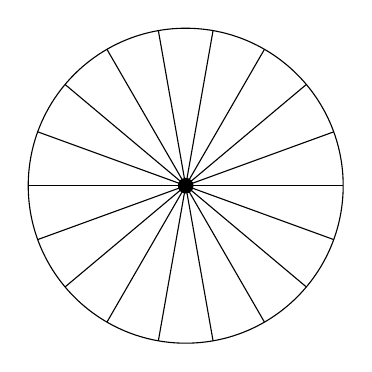
\begin{tikzpicture}
    \draw (0,0) circle (2cm);
    \foreach \x in {0,20,...,350}
      \draw[\OPTblue] (0,0) -- (\x:2cm);
    \node[\OPTblue,circle,fill,inner sep=2pt] (hub) at (0,0) {};
  \end{tikzpicture}
  \caption{一个由轮毂和辐条构成的2维圆盘}
  \label{fig:hub-and-spokes}
\end{figure}

我们可以利用这一想法，将包含$n>1$维道路构造子的高阶归纳类型，用仅包含1维道路构造子的高阶归纳类型来表达。
关键在于，$n$维道路可以表示为一族以某个$(n-1)$维对象为参数的1维道路的连续族。
用于此目的的最简单的$(n-1)$维对象是$(n-1)$维球面，尽管在某些情况下使用其他对象可能更合适。
（回想在\cref{sec:suspension}中，我们能够利用悬垂来归纳地定义球面，而悬垂只涉及1维道路构造子。
事实上，悬垂也可以看作这一想法的一个实例，因为它包含了一族以被悬垂的类型为参数的1维道路。）

\index{torus}
例如，上一节中的环面$T^2$也可以定义为由以下元素生成：


\begin{itemize}
\item 一个点 $b:T^2$，
\item 一条道路 $p:b=b$，
\item 另一条道路 $q:b=b$，
\item 一个点 $h:T^2$，以及
\item 对于每个 $x:\Sn^1$，一条道路 $s(x) : f(x)=h$，其中 $f:\Sn^1\to T^2$ 由 $f(\base)\defeq b$ 和 $\ap f \lloop \defid p \ct q \ct \opp p \ct \opp q$ 定义。
\end{itemize}


这一版本的环面的归纳原理表明，给定 $P:T^2\to\type$，要定义一个截面 $\prd{x:T^2} P(x)$，需要：


\begin{itemize}
\item 一个点 $b':P(b)$，
\item 一条道路 $p' : \dpath P p {b'} {b'}$，
\item 一条道路 $q' : \dpath P q {b'} {b'}$，
\item 一个点 $h':P(h)$，以及
\item 对于每个 $x:\Sn^1$，一条道路 $\dpath {P}{s(x)}{g(x)}{h'}$，其中 $g:\prd{x:\Sn^1} P(f(x))$ 由 $g(\base)\defeq b'$ 和 $\apd g \lloop \defid t(p' \ct q' \ct \opp{(p')} \ct \opp{(q')})$ 定义。
  在后一项中，$\ct$ 表示依值道路的拼接，而 $t:\eqv{(\dpath{P}{\ap f \lloop}{b'}{b'})}{(\dpath{P\circ f}{\lloop}{b'}{b'})}$ 的定义留给读者。
\end{itemize}


注意，这里不需要依值2-道路或$\apdtwofunc{}$。计算规则也留待读者写出。

\begin{rmk}\label{rmk:spokes-no-hub}
有人可能会质疑引入轮毂点$h$的必要性；为什么不能像\cref{fig:spokes-no-hub}所示的那样，简单地添加道路将圆盘的边界连续地连接到边界\emph{上}的某个点呢？
然而，若不作进一步修改，这是行不通的。
因为如果给定某个 $f:\Sn^1 \to X$，我们给出一个道路构造子将每个 $f(x)$ 连接到 $f(\base)$，那么最终得到的结构会更像\cref{fig:spokes-no-hub-ii}中的图形：一个锥，其顶点被扭转并粘合到了底面的某一点上。
问题在于，这样指定的从 $f(\base)$ 到自身的道路可能不是自反性。
我们可以添加一个2维道路构造子来确保这一点，从而补救该问题，但使用一个独立的轮毂点则无需任何高于~1维的道路构造子。
\end{rmk}

\begin{figure}
  \centering
  \begin{minipage}{2in}
    \begin{center}
      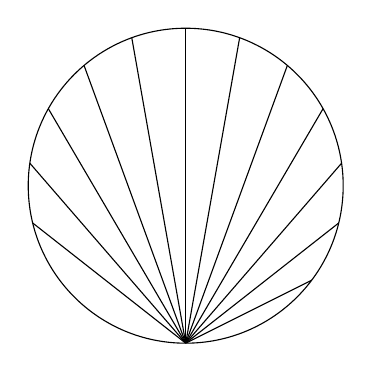
\begin{tikzpicture}
        \draw (0,0) circle (2cm);
        \clip (0,0) circle (2cm);
        \foreach \x in {0,15,...,165}
        \draw[\OPTblue] (0,-2cm) -- (\x:4cm);
      \end{tikzpicture}
    \end{center}
    \caption{无轮毂辐条}
    \label{fig:spokes-no-hub}
  \end{minipage}
  \qquad
  \begin{minipage}{2in}
    \begin{center}
      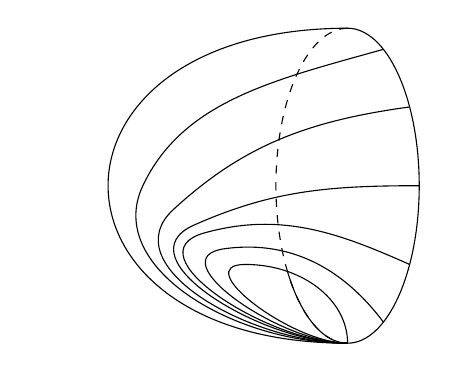
\begin{tikzpicture}[xscale=1.3]
        \draw (0,0) arc (-90:90:.7cm and 2cm) ;
        \draw[dashed] (0,4cm) arc (90:270:.7cm and 2cm) ;
        \draw[\OPTblue] (0,0) to[out=90,in=0] (-1,1) to[out=180,in=180] (0,0);
        \draw[\OPTblue] (0,4cm) to[out=180,in=180,looseness=2] (0,0);
        \path (0,0) arc (-90:-60:.7cm and 2cm) node (a) {};
        \draw[\OPTblue] (a.center) to[out=120,in=10] (-1.2,1.2) to[out=190,in=180] (0,0);
        \path (0,0) arc (-90:-30:.7cm and 2cm) node (b) {};
        \draw[\OPTblue] (b.center) to[out=150,in=20] (-1.4,1.4) to[out=200,in=180] (0,0);
        \path (0,0) arc (-90:0:.7cm and 2cm) node (c) {};
        \draw[\OPTblue] (c.center) to[out=180,in=30] (-1.5,1.5) to[out=210,in=180] (0,0);
        \path (0,0) arc (-90:30:.7cm and 2cm) node (d) {};
        \draw[\OPTblue] (d.center) to[out=190,in=50] (-1.7,1.7) to[out=230,in=180] (0,0);
        \path (0,0) arc (-90:60:.7cm and 2cm) node (e) {};
        \draw[\OPTblue] (e.center) to[out=200,in=70] (-2,2) to[out=250,in=180] (0,0);
        \clip (0,0) to[out=90,in=0] (-1,1) to[out=180,in=180] (0,0);
        \draw (0,4cm) arc (90:270:.7cm and 2cm) ;
      \end{tikzpicture}
    \end{center}
    \caption{无轮毂辐条 II}
    \label{fig:spokes-no-hub-ii}
  \end{minipage}
\end{figure}

\begin{rmk}
  \index{computation rule!propositional}%
  还需注意，这种将高阶道路“转化”为 1-道路的做法，并不能保持这些道路的\emph{判断式}计算规则，尽管它确实能保持\emph{命题式}计算规则。
\end{rmk}

\index{cell complex|)}%
\index{CW complex|)}%

\index{hub and spoke|)}%

\section{推出}
\label{sec:colimits}

\index{type!limit}%
\index{type!colimit}%
\index{limit!of types}%
\index{colimit!of types}%
从范畴论的观点来看，任何基础系统的一个重要方面都在于能够构造极限与余极限。
在集合论基础中，这些是集合的极限与余极限；而在我们的理论里，它们则是\emph{类型}的极限与余极限。
我们已经在 \cref{sec:universal-properties} 中看到，Cartesian 积类型具有作为类型范畴积的正确泛性质，并且在 \cref{ex:coprod-ump} 中看到，余积类型同样具有其预期的泛性质。

如 \cref{sec:universal-properties} 所述，更一般的极限可以利用相等类型与 $\Sigma$ 类型来构造，例如 $f:A\to C$ 与 $g:B\to C$ 的\index{pullback}拉回是 $\sm{a:A}{b:B} (f(a)=g(b))$（参见 \cref{ex:pullback}）。
然而，构造更一般的\emph{余极限}则需要将来自不同类型的元素等同起来，而高阶归纳类型恰好适用于此。
由于我们所有的构造都是同伦不变的，所有的余极限必然都是\emph{同伦余极限}；但为简洁起见，我们省略这一随处可见的修饰语。

本节我们讨论\emph{推出}，它大概是最简单的、也是最有用的余极限之一。
事实上，人们预期所有有限余极限（对于一个恰当的同伦意义上的“有限”定义而言）都可以由推出与有限余积构造出来。
使用高阶归纳类型直接构造更一般的余极限也是可能的，但这有些技术性，且并不完全令人满意，因为我们尚无一个良好的、完全一般的同伦相干图表概念。

\indexsee{type!pushout of}{pushout}%
\index{pushout|(defstyle}%
\index{span}%
给定类型与函数的一个伸展：
\[\Ddiag=\;\vcenter{\xymatrix{C \ar^g[r] \ar_f[d] & B \\ A & }}\]
该伸展的\define{推出}是以下数据所呈现的高阶归纳类型 $A\sqcup^CB$：
\begin{itemize}
\item 一个函数 $\inl:A\to A\sqcup^CB$，
\item 一个函数 $\inr:B \to A\sqcup^CB$，以及
\item 对每个 $c:C$，一条道路 $\glue(c):(\inl(f(c))=\inr(g(c)))$。
\end{itemize}

换句话说，$A\sqcup^CB$ 是 $A$ 与 $B$ 的不交并，再加上对每个 $c:C$ 的一个证据，证明 $f(c)$ 与 $g(c)$ 相等。
递归原理表明，若 $D$ 是另一个类型，我们可以通过定义以下数据来给出映射 $s:A\sqcup^CB\to{}D$：
\begin{itemize}
\item 对每个 $a:A$，$s(\inl(a)):D$ 的值，
\item 对每个 $b:B$，$s(\inr(b)):D$ 的值，以及
\item 对每个 $c:C$，$\mapfunc{s}(\glue(c)):s(\inl(f(c)))=s(\inr(g(c)))$ 的值。
\end{itemize}

我们将归纳原理的表述留给读者。
它还蕴含着下述唯一性原理：如果 $s,s':A\sqcup^CB\to{}D$ 是两个映射，使得
\index{uniqueness!principle, propositional!for functions on a pushout}%
\begin{align*}
  s(\inl(a))&=s'(\inl(a))\\
  s(\inr(b))&=s'(\inr(b))\\
  \mapfunc{s}(\glue(c))&=\mapfunc{s'}(\glue(c))
  \qquad\text{(modulo the previous two equalities)}
\end{align*}
对每个 $a,b,c$ 成立，那么 $s=s'$。

为了表述推出的泛性质，我们引入下述定义。

\begin{defn}\label{defn:cocone}
  给定一个伸展 $\Ddiag= (A \xleftarrow{f} C \xrightarrow{g} B)$ 和一个类型 $D$，一个\define{在伸展 $\Ddiag$ 下、以 $D$ 为顶点的上锥（cocone under $\Ddiag$ with vertex $D$）}
  \indexdef{cocone}%
  \index{vertex of a cocone}%
  由函数 $i:A\to{}D$ 和 $j:B\to{}D$ 以及一个同伦 $h : \prd{c:C} (i(f(c))=j(g(c)))$ 组成：
  \[\uppercurveobject{{ }}\lowercurveobject{{ }}\twocellhead{{ }}
  \xymatrix{C \ar^g[r] \ar_f[d] \drtwocell{^h} & B \ar^j[d] \\ A \ar_i[r] & D
  }\]
  我们用 $\cocone{\Ddiag}{D}$ 表示所有这类上锥的类型，即
  \[ \cocone{\Ddiag}{D} \defeq
  \sm{i:A\to D}{j:B\to D} \prd{c:C} (i(f(c))=j(g(c))).
  \]
\end{defn}

显然，存在一个在 $\Ddiag$ 下以 $A\sqcup^C B$ 为顶点的典范上锥，它由 $\inl$、$\inr$ 和 $\glue$ 组成。
\[\uppercurveobject{{ }}\lowercurveobject{{ }}\twocellhead{{ }}
\xymatrix{C \ar^g[r] \ar_f[d] \drtwocell{^\glue\ \ } & B \ar^{\inr}[d] \\
  A \ar_-\inl[r] & A\sqcup^CB }\]
下述引理说明，这个上锥是万有上锥。

\begin{lem}\label{thm:pushout-ump}
  \index{universal!property!of pushout}%
  对任意类型 $E$，存在一个等价
  \[ (A\sqcup^C B \to E) \;\eqvsym\; \cocone{\Ddiag}{E}. \]
\end{lem}

\begin{proof}
  考虑任意类型 $E:\type$。
  有一个典范函数 $c_\sqcup$，其定义为
  \[\function{(A\sqcup^CB\to{}E)}{\cocone{\Ddiag}{E}}
  {t}{(t\circ{}\inl,t\circ{}\inr,\mapfunc{t}\circ{}\glue)}\]
  我们非正式地将这个函数记作 $t\mapsto\composecocone{t}c_\sqcup$。
  我们将证明这是一个等价。

  首先，给定一个 $c=(i,j,h):\cocone{\mathscr{D}}{E}$，我们需要构造一个从 $A\sqcup^CB$ 到 $E$ 的映射 $\mathsf{s}(c)$。
  \[\uppercurveobject{{ }}\lowercurveobject{{ }}\twocellhead{{ }}
  \xymatrix{C \ar^g[r] \ar_f[d] \drtwocell{^h} & B \ar^{j}[d] \\
    A \ar_-{i}[r] & E }\]
  映射 $\mathsf{s}(c)$ 按以下方式定义
  \begin{align*}
    \mathsf{s}(c)(\inl(a))&\defeq i(a),\\
    \mathsf{s}(c)(\inr(b))&\defeq j(b),\\
    \mapfunc{\mathsf{s}(c)}(\glue(x))&\defid h(x).
  \end{align*}
我们定义了一个映射
\[\function{\cocone{\Ddiag}{E}}{(A\sqcup^CB\to{}E)}{c}{\mathsf{s}(c)}\]
现在需要证明这个映射是
$t\mapsto{}\composecocone{t}c_\sqcup$
的逆。
一方面，如果 $c=(i,j,h):\cocone{\Ddiag}{E}$，我们有
\begin{align*}
  \composecocone{\mathsf{s}(c)}c_\sqcup & =
  (\mathsf{s}(c)\circ\inl,\mathsf{s}(c)\circ\inr,
  \mapfunc{\mathsf{s}(c)}\circ\glue) \\
  & = (\lamu{a:A} \mathsf{s}(c)(\inl(a)),\;
  \lamu{b:B} \mathsf{s}(c)(\inr(b)),\;
  \lamu{x:C} \mapfunc{\mathsf{s}(c)}(\glue(x))) \\
  & = (\lamu{a:A} i(a),\;
  \lamu{b:B} j(b),\;
  \lamu{x:C} h(x)) \\
  & \jdeq (i, j, h) \\
  & = c.
\end{align*}
%
另一方面，如果 $t:A\sqcup^CB\to{}E$，我们希望证明
$\mathsf{s}(\composecocone{t}c_\sqcup)=t$。
对于 $a:A$，我们有
\[\mathsf{s}(\composecocone{t}c_\sqcup)(\inl(a))=t(\inl(a))\]
因为 $\composecocone{t}c_\sqcup$ 的第一个分量是 $t\circ\inl$。
同样地，对于 $b:B$ 我们有
\[\mathsf{s}(\composecocone{t}c_\sqcup)(\inr(b))=t(\inr(b))\]
而对于 $x:C$ 我们有
\[\mapfunc{\mathsf{s}(\composecocone{t}c_\sqcup)}(\glue(x))
=\mapfunc{t}(\glue(x))\]
因此 $\mathsf{s}(\composecocone{t}c_\sqcup)=t$。

这就证明了 $c\mapsto\mathsf{s}(c)$ 是 $t\mapsto{}\composecocone{t}c_\sqcup$ 的拟逆，符合要求。
\end{proof}

许多标准的同伦论构造都可以表示为（同伦）推出。


\begin{itemize}
\item 伸展 $\unit \leftarrow A \to \unit$ 的推出是\define{纬悬（suspension）} $\susp A$（参见 \cref{sec:suspension}）。%
  \index{suspension}
\symlabel{join}
\item $A \xleftarrow{\proj1} A\times B \xrightarrow{\proj2} B$ 的推出称为 $A$ 和 $B$ 的\define{联结（join）}，记作 $A*B$。%
  \indexdef{join!of types}
\item $\unit \leftarrow A \xrightarrow{f} B$ 的推出是 $f$ 的\define{锥（cone）}或\define{余纤维（cofiber）}。%
  \indexdef{cone!of a function}%
  \indexsee{mapping cone}{cone of a function}%
  \indexdef{cofiber of a function}%
\symlabel{wedge}
\item 如果 $A$ 和 $B$ 分别配有基点 $a_0:A$ 和 $b_0:B$，那么 $A \xleftarrow{a_0} \unit \xrightarrow{b_0} B$ 的推出是\define{楔（wedge）} $A\vee B$。%
  \indexdef{wedge}
\symlabel{smash}
\item 如果 $A$ 和 $B$ 如前所述带点，由 $f(\inl(a))\defeq (a,b_0)$ 和 $f(\inr(b))\defeq (a_0,b)$ 定义 $f:A\vee B \to A\times B$，并满足 $\ap f \glue \defid \refl{(a_0,b_0)}$。
  那么 $f$ 的锥称为\define{缩积（smash product）} $A\wedge B$。%
  \indexdef{smash product}
\end{itemize}


我们将在 \cref{cha:hlevels,cha:homotopy} 中进一步讨论推出。

\begin{rmk}
  如 \cref{subsec:prop-trunc} 所述，符号 $\wedge$ 和 $\vee$ 既用于表示带点空间的缩积和楔，也用于逻辑中的``与''和``或''。
  由于同伦类型论中的类型既可以表现得像空间，也可以表现得像命题，从技术上讲，存在潜在的冲突——但由于它们很少同时扮演两种角色，语境通常能消除歧义。
  此外，缩积和楔仅适用于\emph{带点}空间，而唯一带点的命题是 $\top\jdeq\unit$——并且无论 $\wedge$ 和 $\vee$ 取哪种含义，都有 $\unit\wedge \unit = \unit$ 和 $\unit\vee\unit=\unit$。
\end{rmk}

\index{pushout|)}%

\begin{rmk}
  需要注意的是，余极限一般不保持截断性质。
  例如，$\Sn^0$ 和 \unit 都是集合，但 $\unit \leftarrow \Sn^0 \to \unit$ 的推出是 $\Sn^1$，而 $\Sn^1$ 不是集合。
  因此，如果我们对 $n$-类型范畴（特别是集合范畴）中的余极限感兴趣，就需要以某种方式对余极限进行``截断''。
  我们将在 \cref{sec:hittruncations,cha:hlevels,cha:set-math} 中回到这一点。
\end{rmk}

\section{截断}
\label{sec:hittruncations}

\index{truncation!propositional|(}%
在 \cref{subsec:prop-trunc} 中，我们将命题截断作为一种新的类型形成操作引入；
现在我们可以观察到，它可以作为高阶归纳类型的一个特例而得到。
这将理解截断的问题化归为理解高阶归纳类型的问题，而后者至少是可以通过系统方法来处理的。
这一点也很有趣，因为它提供了我们的第一个真正\emph{递归}的高阶归纳类型的例子，因为其构造子的输入取自正被定义的类型本身（就像后继函数 $\suc:\nat\to\nat$ 那样）。

设 $A$ 是一个类型；我们定义其命题截断 $\brck A$ 为由以下生成的高阶归纳类型：

\begin{itemize}
\item 一个函数 $\bprojf : A \to \brck A$，以及
\item 对于每个 $x,y:\brck A$，一条道路 $x=y$。
\end{itemize}

注意，第二个构造子所定义的正是 $\brck A$ 为纯粹命题这一断言。
因此，$\brck A$ 的定义可以这样理解：$\brck A$ 由一个函数 $A\to\brck A$ 连同它是纯粹命题这一事实\emph{自由生成}。

这个高阶归纳定义的递归原理不难写出：给定任意类型 $B$ 及以下条件

\begin{itemize}
\item 一个函数 $g:A\to B$，以及
\item 对于任意 $x,y:B$，都有一条道路 $x=_B y$，
\end{itemize}

则存在函数 $f:\brck A \to B$，使得

\begin{itemize}
\item 对所有 $a:A$，有 $f(\bproj a) \jdeq g(a)$，且
\item 对于任意 $x,y:\brck A$，函数 $\apfunc f$ 将 $\brck A$ 中指定的道路 $x=y$ 映到 $B$ 中指定的道路 $f(x) = f(y)$（在命题层面）。
\end{itemize}

\index{recursion principle!for truncation}%
这些正是我们在 \cref{subsec:prop-trunc} 中为命题截断的递归原理所陈述的前提——即一个函数 $A\to B$，其中 $B$ 是纯粹命题——且结论的第一部分也与我们那里的陈述完全一致。
第二部分（$\apfunc f$ 的作用）之前并未提及，但在此情形下它实际上是空洞的，因为 $B$ 是纯粹命题，所以其中的\emph{任意}两条道路都自动相等。

\index{induction principle!for truncation}%
$\brck A$ 同样有归纳原理：给定任意 $B:\brck A \to \type$ 及以下条件

\begin{itemize}
\item 一个函数 $g:\prd{a:A} B(\bproj a)$，以及
\item 对于任意 $x,y:\brck A$，$u:B(x)$ 和 $v:B(y)$，都有一条依值道路 $q:\dpath{B}{p(x,y)}{u}{v}$，其中 $p(x,y)$ 是来自 $\brck A$ 第二个构造子的道路，
\end{itemize}

则存在 $f:\prd{x:\brck A} B(x)$，使得对 $a:A$ 有 $f(\bproj a)\jdeq g(a)$，并且还有另一条计算规则。
然而，由于任意两个纯粹命题之间（在同伦意义下）至多只有一个函数，这个归纳原理其实并不太有用（另见 \cref{ex:prop-trunc-ind}）。

\index{truncation!propositional|)}%
\index{truncation!set|(}%

\index{set|(}%
不过，我们可以将这一想法推广，对任意 $n$，构造出类似的落在 $n$-类型中的截断。
例如，我们可以将\emph{$0$-截断} $\trunc0A$ 定义为由以下内容生成：

\begin{itemize}
\item 一个函数 $\tprojf0 : A \to \trunc0 A$，以及
\item 对于每对 $x,y:\trunc0A$ 及每对道路 $p,q:x=y$，都有一条道路 $p=q$。
\end{itemize}

那么，$\trunc0A$ 就是由一个函数 $A\to \trunc0A$ 连同``$\trunc0A$ 是集合''这一断言自由生成的。
它的一个自然的归纳原理是说：给定 $B:\trunc0 A \to \type$ 及以下条件

\begin{itemize}
\item 一个函数 $g:\prd{a:A} B(\tproj0a)$，以及
\item 对于任意 $x,y:\trunc0A$，$z:B(x)$ 和 $w:B(y)$，以及每对道路 $p,q:x=y$ 满足 $r:\dpath{B}{p}{z}{w}$ 和 $s:\dpath{B}{q}{z}{w}$，都有一条 $2$-道路 $v:\dpath{\dpath{B}{-}{z}{w}}{u(x,y,p,q)}{r}{s}$，其中 $u(x,y,p,q):p=q$ 得自 $\trunc0A$ 的第二个构造子，
\end{itemize}

则存在 $f:\prd{x:\trunc0A} B(x)$，使得对所有 $a:A$ 有 $f(\tproj0a)\jdeq g(a)$，并且 $\apdtwo{f}{u(x,y,p,q)}$ 就是上面指定的那条 $2$-道路。
（与命题截断的情形一样，后一个条件实际上是无趣的。）
然而，由此出发，我们可以证明一个更有用的归纳原理。

\begin{lem}\label{thm:trunc0-ind}
  假设给定 $B:\trunc0 A \to \type$ 及 $g:\prd{a:A} B(\tproj0a)$，并且每个 $B(x)$ 都是集合。
  则存在 $f:\prd{x:\trunc0A} B(x)$，使得对所有 $a:A$ 都有 $f(\tproj0a)\jdeq g(a)$。
\end{lem}

\begin{proof}
  只需对如上所述的任意 $x,y,z,w,p,q,r,s$ 构造一条 $2$-道路 $v:\dpath{B}{u(x,y,p,q)}{r}{s}$ 即可。
  然而，根据依值 $2$-道路的定义，这是纤维 $B(y)$ 中的一条普通 $2$-道路。
  由于 $B(y)$ 是集合，任意两条平行道路之间都存在 $2$-道路。
\end{proof}

这蕴含了所期望的泛性质。

\begin{lem}\label{thm:trunc0-lump}
  \index{universal!property!of truncation}%
  对于任意集合 $B$ 和任意类型 $A$，与 $\tprojf0:A\to \trunc0A$ 复合确定了一个等价
  \[ \eqvspaced{(\trunc0A\to B)}{(A\to B)}. \]
\end{lem}

\begin{proof}
  将 \cref{thm:trunc0-ind} 应用于常值族这一特殊情形，得到一个从右到左的映射，它是从左到右``与 $\tprojf0$ 复合''映射的右逆。
  为证明它也是左逆，任取 $h:\trunc0A\to B$，并将 \cref{thm:trunc0-ind} 应用于复合 $a\mapsto h(\tproj0a)$ 来定义 $h':\trunc0A\to B$。
  于是有 $h'(\tproj0a)=h(\tproj0a)$。

  然而，由于 $B$ 是集合，对于任意 $x:\trunc0A$，类型 $h(x)=h'(x)$ 是纯粹命题，因而也是集合。
  于是，由 \cref{thm:trunc0-ind}，对任意 $a:A$ 有 $h'(\tproj0a)=h(\tproj0a)$ 这一观察蕴含了对任意 $x:\trunc0A$ 都有 $h(x)=h'(x)$，从而 $h=h'$。
\end{proof}

\index{limit!of sets}%
\index{colimit!of sets}%
例如，这使我们能够构造集合的余极限。
我们已经看到，如果 $A \xleftarrow{f} C \xrightarrow{g} B$ 是集合的一个伸展，那么推出 $A\sqcup^C B$ 可能不再是集合。
（例如，若 $A$ 和 $B$ 都是 \unit 而 $C$ 是 \bool，则推出是 $\Sn^1$。）
然而，我们可以通过截断，构造出一个作为集合的推出，并且它对其他集合具有预期的泛性质。

\begin{lem}\label{thm:set-pushout}
  \index{universal!property!of pushout}%
  设 $A \xleftarrow{f} C \xrightarrow{g} B$ 是集合的一个伸展\index{span}。
  那么对任意集合 $E$，存在一个典范等价
  \[ \Parens{\trunc0{A\sqcup^C B} \to E} \;\eqvsym\; \cocone{\Ddiag}{E}. \]
\end{lem}

\begin{proof}
  组合 \cref{thm:pushout-ump,thm:trunc0-lump} 中的等价即得。
\end{proof}

我们将 $\trunc0{A\sqcup^C B}$ 称为 $f$ 与 $g$ 的 \define{集合推出}
\indexdef{set-pushout}%
\index{pushout!of sets}，
以区别于（同伦）推出 $A\sqcup^C B$。
或者，我们也可以修改 \cref{sec:colimits} 中推出的定义，直接加入 $0$-截断构造子，从而避免事后再做截断。
类似的说明适用于任何一种集合余极限；我们将在 \cref{cha:set-math} 中进一步探讨这一点。

然而，尽管上述 $0$-截断的定义是可行的——它给出了我们期望的结果，并且是相容的——但它存在一些问题。
首先，它不能很好地融入高阶归纳类型的一般理论。
一般来说，直接处理像 $\trunc0A$ 的第二个构造子那样的构造子是很棘手的，因为它的\emph{输入}不仅涉及被定义类型的元素，还涉及其中的道路。

不过，这个问题可以比较容易地解决。
回想一下，在 \cref{sec:bool-nat} 中我们提到，可以通过让一个构造子接受一个类型为 $\nat\to W$ 的单个参数，从而允许归纳类型 $W$ 的构造子接受“无限多个”类型为 $W$ 的参数。
这背后有一个一般性原则：要为输入形式古怪的构造子建模，可以使用一个辅助的归纳类型（例如 \nat）来参数化它们，从而将输入化为一个以归纳类型为定义域的简单函数。

对于 $0$-截断，我们可以考虑辅助的\emph{高阶}归纳类型 $S$，它由两个点 $a,b:S$ 和两条道路 $p,q:a=b$ 生成。
那么，$\trunc 0A$ 那个略显可疑的构造子就可以替换为下面这个毫无问题的构造子：


\begin{itemize}
\item 对每个 $f:S\to \trunc 0A$，一条道路 $\apfunc{f}(p) = \apfunc{f}(q)$。
\end{itemize}


因为给出一个从 $S$ 出发的映射，相当于给出两个点以及它们之间的两条平行道路，所以这导出了相同的归纳原理。

\index{set|)}%

\index{truncation!set|)}%
\index{truncation!n-truncation@$n$-truncation}%
然而，我们当前 $0$-截断定义的一个更严重的问题是，它不太容易推广。
如果我们想为所有 $n:\nat$ 统一地描述一种将类型“$n$-截断”到 $n$-类型的定义方式，那么当前的方法是行不通的，因为第二个构造子所需的参数个数会随 $n$ 的增大而增加。
因此，在 \cref{sec:truncations} 中，我们将基于上面引入的类型 $S$ 等价于圆 $\Sn^1$ 这一观察，采用不同的想法来构造这些截断。
这一方法将 $0$-截断作为特例包含在内，并且满足 \cref{thm:trunc0-ind,thm:trunc0-lump} 的推广版本。

\section{商}
\label{sec:set-quotients}

集合的一种特别重要的余极限是按\emph{关系}取的\emph{商}。
也就是说，设 $A$ 是一个集合，且 $R:A\times A \to \prop$ 是一个命题族（一个\define{纯粹关系}）。
\indexdef{relation!mere}%
\indexdef{mere relation}%
它的商应该是两个投影
\[ \tsm{a,b:A} R(a,b) \rightrightarrows A. \]
的集合余等子。
我们也可以直接将其描述为高阶归纳类型 $A/R$，它由以下内容生成：
\index{set-quotient|(defstyle}%
\indexsee{quotient of sets}{set-quotient}%
\indexsee{type!quotient}{set-quotient}%


\begin{itemize}
\item 一个函数 $q:A\to A/R$；
\item 对每个满足 $R(a,b)$ 的 $a,b:A$，一个相等 $q(a)=q(b)$；以及
\item $0$-截断构造子：对所有 $x,y:A/R$ 和 $r,s:x=y$，有 $r=s$。
\end{itemize}


我们有时会将这个高阶归纳类型 $A/R$ 称为 $A$ 按 $R$ 的 \define{集合商}，以强调它按定义产生一个集合。
（在同伦论中存在更一般的“商”的概念，但它们大多超出了本书的范围。不过，在 \cref{sec:rezk} 中，我们将考虑类型按 $1$-群胚取“商”的情形，这是比集合商更高一层的构造。）

\begin{rmk}\label{rmk:quotient-of-non-set}
  对于集合商的定义及其大多数性质而言，$A$ 实际上并不一定需要是集合。
  不过，集合的情形通常最受关注。
\end{rmk}

\begin{lem}\label{thm:quotient-surjective}
  函数 $q:A\to A/R$ 是满的。
\end{lem}

\begin{proof}
  我们需要证明，对于任何 $x:A/R$，都仅仅存在一个 $a:A$ 使得 $q(a)=x$。
  我们使用 $A/R$ 的归纳原理。
  第一种情况是平凡的：如果 $x$ 是 $q(a)$，那么当然仅仅存在一个 $a$ 使得 $q(a)=q(a)$。
  由于目标是一个命题，它自动尊重所有道路构造子，因此我们就证完了。
\end{proof}

现在我们可以证明，集合商具有所期望的（集合）余等子的泛性质。

\begin{lem}\label{thm:quotient-ump}
  对于任何集合 $B$，与 $q$ 预复合给出一个等价：
  \[ \eqvspaced{(A/R \to B)}{\Parens{\sm{f:A\to B} \prd{a,b:A} R(a,b) \to (f(a)=f(b))}}.\]
\end{lem}

\begin{proof}
  $\blank\circ q$ 的拟逆（从右到左）就是 $A/R$ 的递归原理。
  也就是说，给定 $f:A\to B$ 使得
  \narrowequation{\prd{a,b:A} R(a,b) \to (f(a)=f(b)),} 我们通过 $\bar f(q(a))\defeq f(a)$ 来定义 $\bar f:A/R\to B$。
  这个定义方程说的正是 $(f\mapsto \bar f)$ 是 $(\blank\circ q)$ 的一个右逆。

  要证明它同时也是左逆，我们必须证明对于任意 $g:A/R\to B$ 和 $x:A/R$ 有 $g(x) = \overline{g\circ q}(x)$。
  然而，根据 \cref{thm:quotient-surjective}，仅仅存在 $a$ 使得 $q(a)=x$。
  由于我们欲证的相等是一个命题，我们可以假设确实存在这样的 $a$，此时便有 $g(x) = g(q(a)) = \overline{g\circ q}(q(a)) = \overline{g\circ q}(x)$。
\end{proof}

当然，经典数学中通常考虑的情况是 $R$ 为一个\define{等价关系（equivalence relation）}，即我们有
\indexdef{relation!equivalence}%
\indexsee{equivalence!relation}{relation, equivalence}%
%


\begin{itemize}
\item \define{自反性（reflexivity）}：$\prd{a:A} R(a,a)$，
  \indexdef{reflexivity!of a relation}%
  \indexdef{relation!reflexive}%
\item \define{对称性（symmetry）}：$\prd{a,b:A} R(a,b) \to R(b,a)$，以及
  \indexdef{symmetry!of a relation}%
  \indexdef{relation!symmetric}%
\item \define{传递性（transitivity）}：$\prd{a,b,c:C} R(a,b) \times R(b,c) \to R(a,c)$。
  \indexdef{transitivity!of a relation}%
  \indexdef{relation!transitive}%
\end{itemize}


%
此时，集合商 $A/R$ 将具备更多良好的性质，我们将在 \cref{sec:piw-pretopos} 中看到：例如，我们有 $R(a,b) \eqvsym (\id[A/R]{q(a)}{q(b)})$。
\symlabel{equivalencerelation}
我们通常将等价关系 $R(a,b)$ 写作中缀形式 $a\eqr b$。

等价关系的商也可以用其他方式构造。
集合论的方法是考虑等价类构成的集合，作为 $A$ 的幂集\index{power set}的一个子集。
我们也可以在类型论中模仿这种``非直谓''的构造。
\index{impredicative!quotient}

\begin{defn}
  一个谓词 $P:A\to\prop$ 是关系 $R : A \times A \to \prop$ 的一个\define{等价类（equivalence class）}
  \indexdef{equivalence!class}%
  如果仅仅存在一个 $a:A$，使得对所有的 $b:A$ 有 $\eqv{R(a,b)}{P(b)}$。
\end{defn}

由于 $R$ 和 $P$ 都是命题，等价 $\eqv{R(a,b)}{P(b)}$ 与蕴含 $R(a,b) \to P(b)$ 和 $P(b) \to R(a,b)$ 是一回事。
当然，对于任何 $a:A$，我们有典范的等价类 $P_a(b) \defeq R(a,b)$。

\begin{defn}\label{def:VVquotient}
  我们定义
  \begin{equation*}
    A\sslash R \defeq \setof{ P:A\to\prop | P \text{ is an equivalence class of } R}.
  \end{equation*}
  函数 $q':A\to A\sslash R$ 定义为 $q'(a) \defeq P_a$。
\end{defn}

\begin{thm}
  对于 $A$ 上的任意等价关系 $R$，类型 $A\sslash R$ 等价于集合商 $A/R$。
\end{thm}

\begin{proof}
  首先注意，如果 $R(a,b)$，那么由于 $R$ 是等价关系，对于任何 $c:A$ 我们有 $R(a,c) \Leftrightarrow R(b,c)$。
  因此，根据泛等性有 $R(a,c) = R(b,c)$，再由函数外延性即得 $P_a=P_b$，也就是说 $q'(a)=q'(b)$。
  于是，由 \cref{thm:quotient-ump} 我们得到一个诱导映射 $f:A/R \to A\sslash R$，满足 $f\circ q = q'$。

  我们证明 $f$ 既是单的又是满的，从而是一个等价。
  满射性直接由 $q'$ 是满的得出，而 $q'$ 的满射性本质上由 $A\sslash R$ 的定义保证。
  对于单射性，如果 $f(x)=f(y)$，为了证明命题 $x=y$，根据 $q$ 的满射性，我们可以假设存在 $a,b:A$ 使得 $x=q(a)$ 且 $y=q(b)$。
  那么对于任意 $c:A$ 有 $R(a,c) = f(q(a))(c) = f(q(b))(c) = R(b,c)$，特别地有 $R(a,b) = R(b,b)$。
  但由于 $R$ 是等价关系，$R(b,b)$ 是有实例的，故而 $R(a,b)$ 也有实例。
  因此 $q(a)=q(b)$，即 $x=y$。
\end{proof}

在 \cref{subsec:quotients} 中，我们将给出这个定理的另一个证明。
请注意，与 $A/R$ 不同，构造 $A\sslash R$ 会提升宇宙层级：如果 $A:\UU_i$ 且 $R:A\to A\to \prop_{\UU_i}$，那么在定义 $A\sslash R$ 时，我们也必须使用 $\prop_{\UU_i}$ 来包含所有等价类，因此 $A\sslash R : \UU_{i+1}$。
当然，如果我们假设 \cref{subsec:prop-subsets} 中的命题大小重整公理，就可以避免这个问题。

\begin{rmk}\label{defn-Z}
前面的两种构造提供了一般性的商构造，但在某些具体情形下，可能存在更简单的构造。
例如，我们可以将整数 \Z 定义为一个集合商
\indexdef{integers}%
\indexdef{number!integers}%
%
\[ \Z \defeq (\N \times \N)/{\eqr} \]
%
其中 $\eqr$ 是由下式定义的等价关系：
%
\[ (a,b) \eqr (c,d) \defeq (a + d = b + c). \]
%
换言之，一对数 $(a,b)$ 代表整数 $a - b$。
然而，在这种情况下，等价类存在\emph{典范代表元（canonical representatives）}：形如 $(n,0)$ 或 $(0,n)$ 的那些对。
\end{rmk}

以下引理表明，当出现这类情况时，我们就不再需要前面任何一种通用的商构造了。
（一个函数 $r:A\to A$ 如果满足 $r\circ r = r$，则称之为\define{幂等的（idempotent）}
\indexdef{function!idempotent}%
\indexdef{idempotent!function}%
。）

\begin{lem}\label{lem:quotient-when-canonical-representatives}
  设 $\eqr$ 是集合 $A$ 上的一个关系，并且存在一个幂等函数 $r: A \to A$，使得对一切 $x, y: A$ 有 $\eqv{(r(x) = r(y))}{(x \eqr y)}$。
  （这蕴含 $\eqr$ 是一个等价关系。）
  那么类型
  %
  \begin{equation*}
    (A/{\eqr}) \defeq \Parens{\sm{x : A} r(x) = x}
  \end{equation*}
  %
  满足 $A$ 关于 $\eqr$ 的集合商的泛性质，因此与之等价。
  换句话说，存在一个映射 $q : A \to (A/{\eqr})$，使得对于任意集合 $B$，与 $q$ 的预复合诱导出一个等价
  %
  \begin{equation}
    \label{eq:quotient-when-canonical}
    \Parens{(A/{\eqr}) \to B} \eqvsym \Parens{\sm{g : A \to B} \prd{x, y : A} (x \eqr y) \to (g(x) = g(y))}.
  \end{equation}
\end{lem}

\begin{proof}
  令 $i : \prd{x : A} r(r(x)) = r(x)$ 见证 $r$ 的幂等性。
  映射 $q : A \to (A/{\eqr})$ 由 $q(x) \defeq (r(x), i(x))$ 定义。
  注意，由于 $A$ 是集合，我们有 $q(x)=q(y)$ 当且仅当 $r(x)=r(y)$，从而（根据假设）当且仅当 $x \eqr y$。
  我们在\eqref{eq:quotient-when-canonical}中如下定义从左到右的映射 $e$：
  \[ e(f) \defeq (f \circ q, \nameless), \]
  %
  其中下划线 $\nameless$ 表示如下的证明：如果 $x, y : A$ 且 $x \eqr y$，那么如上所述 $q(x)=q(y)$，因此 $f(q(x)) = f(q(y))$。
  为证明 $e$ 是一个等价，考虑反方向的映射 $e'$，其定义为
  %
  \[ e'(g, s) (x,p) \defeq g(x). \]
  %
  给定任意 $f : (A/{\eqr}) \to B$，有
  %
  \[ e'(e(f))(x, p) \jdeq f(q(x)) \jdeq f(r(x), i(x)) = f(x, p) \]
  %
  最后一个等式成立是因为 $p : r(x) = x$，并且由于 $A$ 是集合，我们有 $(x,p) = (r(x), i(x))$。
  类似地，我们计算
  %
  \[ e(e'(g, s)) \jdeq e(g \circ \proj{1}) \jdeq (g \circ \proj{1} \circ q, {\nameless}). \]
  %
  由于 $B$ 是集合，我们不必考虑 $\nameless$ 的部分，而对于第一个分量，我们有
  %
  \[ g(\proj{1}(q(x))) \jdeq g(r(x)) = g(x), \]
  %
  其中最后一个等式成立是因为 $r(x) \eqr x$，而由假设 $s$，$g$ 尊重 $\eqr$。
\end{proof}

\begin{cor}\label{thm:retraction-quotient}
  设 $p:A\to B$ 是集合之间的一个收缩。
  那么 $B$ 是 $A$ 模去由下式定义的等价关系 $\eqr$ 的商：
  \[ (a_1 \eqr a_2) \defeq (p(a_1) = p(a_2)). \]
\end{cor}

\begin{proof}
  设 $s:B\to A$ 是 $p$ 的一个截面。
  那么 $s\circ p : A\to A$ 是一个幂等函数，它关于这个 $\eqr$ 满足 \cref{lem:quotient-when-canonical-representatives} 的条件，并且 $s$ 诱导了从 $B$ 到其不动点集的一个同构。
\end{proof}

\begin{rmk}\label{Z-quotient-by-canonical-representatives}
\cref{lem:quotient-when-canonical-representatives} 可应用于 $\Z$，其中幂等函数 $r : \N \times \N \to \N \times \N$ 定义为
%
\begin{equation*}
  r(a, b) =
  \begin{cases}
    (a - b, 0) & \text{if $a \geq b$,} \\
    (0, b - a) & \text{otherwise.}
  \end{cases}
\end{equation*}
%
（即使构造性地看，这也是一个合法的定义，因为 $\N$ 上的关系 $\geq$ 是可判定的。）
这样，一个非负整数典范地由 $(k, 0)$ 代表，一个非正整数由 $(0, m)$ 代表，其中 $k,m:\N$。
这种分情况处理的方式蕴含着下面这个关于整数的``归纳原理''，它在 \cref{cha:homotopy} 中会很有用。
\index{natural numbers}%
（照例，我们将自然数 $n$ 与相应的非负整数等同，即等同于 $(n,0):\N\times\N$ 在 $\Z$ 中的像。）
\end{rmk}

\begin{lem}\label{thm:sign-induction}
  \index{integers!induction principle for}%
  \index{induction principle!for integers}%
  设 $P:\Z\to\type$ 是一个类型族，并且我们已有
  \begin{itemize}
  \item $d_0: P(0)$，
  \item $d_+: \prd{n:\N} P(n) \to P(\suc(n))$，以及
  \item $d_- : \prd{n:\N} P(-n) \to P(-\suc(n))$。
  \end{itemize}
  那么存在 $f:\prd{z:\Z} P(z)$，使得
  \begin{itemize}
    \item $f(0) = d_0$，
    \item $f(\suc(n)) = d_+(n,f(n))$ 对所有 $n:\N$ 成立，且
    \item $f(-\suc(n)) = d_-(n,f(-n))$ 对所有 $n:\N$ 成立。
  \end{itemize}
\end{lem}

\begin{proof}
  在此证明中，我们令 $\Z$ 表示 $\sm{x:\N\times\N}(r(x)=x)$，其中 $r$ 是上面给出的幂等函数。
  （然后我们可以将结果传输到任何与 $\Z$ 等价的定义上。）
  令 $q:\N\times\N\to\Z$ 为商映射，如 \cref{lem:quotient-when-canonical-representatives} 中那样由 $q(x) = (r(x),i(x))$ 定义。
  现在定义 $Q\defeq P\circ q:\N\times \N \to \type$。
  通过将给定的数据沿适当的等式传输，我们得到
  \begin{align*}
    d'_0 &: Q(0,0)\\
    d'_+ &: \prd{n:\N} Q(n,0) \to Q(\suc(n),0)\\
    d'_- &: \prd{n:\N} Q(0,n) \to Q(0,\suc(n)).
  \end{align*}
  另请注意，由于 $q(n,m) = q(\suc(n),\suc(m))$，我们有一个诱导的等价
  \[e_{n,m}:\eqv{Q(n,m)}{Q(\suc(n),\suc(m))}.\]
  然后我们可以通过对 $x$ 进行双重归纳来构造 $g:\prd{x:\N\times \N} Q(x)$：
  \begin{align*}
    g(0,0) &\defeq d'_0,\\
    g(\suc(n),0) &\defeq d'_+(n,g(n,0)),\\
    g(0,\suc(m)) &\defeq d'_-(m,g(0,m)),\\
    g(\suc(n),\suc(m)) &\defeq e_{n,m}(g(n,m)).
  \end{align*}
  现在我们有 $\proj1 : \Z \to \N\times\N$，且满足 $q\circ \proj1 = \idfunc$。
  因此，特别地，我们有 $Q\circ \proj1 = P$，从而得到一族等价 $s:\prd{z:\Z} \eqv{Q(\proj1(z))}{P(z)}$。
  于是，我们可以定义 $f(z) = s(z,g(\proj1(z)))$ 来得到 $f:\prd{z:\Z} P(z)$，并验证所要求的等式。
\end{proof}

我们有时会用模式匹配语法来表示从 \cref{thm:sign-induction} 得到的函数 $f:\prd{z:\Z} P(z)$，它包含 $d_0$、$d_+$ 和 $d_-$ 这三种情形：
\begin{align*}
  f(0) &\defid d_0\\
  f(\suc(n)) &\defid d_+(n,f(n))\\
  f(-\suc(n)) &\defid d_-(n,f(-n))
\end{align*}
正如我们在处理高阶归纳类型的道路构造子时所做的那样，我们使用 $\defid$ 而非 $\defeq$，以表明由 \cref{thm:sign-induction} 蕴含的``计算''规则仅仅是命题相等性。
例如，通过这种方式，我们可以为任意整数 $n$ 定义一个环路的 $n$ 重拼接。

\begin{cor}\label{thm:looptothe}
  \indexdef{path!concatenation!n-fold@$n$-fold}%
  设 $A$ 是一个类型，$a:A$ 且 $p:a=a$。
  存在一个函数 $\prd{n:\Z} (a=a)$，记作 $n\mapsto p^n$，其定义如下：
  \begin{align*}
    p^0 &\defid \refl{a}\\
    p^{n+1} &\defid p^n \ct p
    & &\text{for $n\ge 0$}\\
    p^{n-1} &\defid p^n \ct \opp p
    & &\text{for $n\le 0$.}
  \end{align*}
\end{cor}

关于整数，我们将在 \cref{sec:free-algebras,sec:field-rati-numb} 作进一步讨论。

\index{set-quotient|)}%

\section{代数}
\label{sec:free-algebras}

高阶归纳类型不仅能用来构造球面、胞腔复形等高维对象，即便仅限于集合的层面，它们也非常有用。
在 \cref{thm:set-pushout} 中我们已经见过一个例子：它们使我们能够构造任意集合图表的余极限，而这在 \cref{cha:typetheory} 的基础类型论中是无法做到的。
当我们研究带有代数结构的集合时，高阶归纳类型同样极为有用。

作为本节贯穿的例子，我们考虑\emph{群（groups）}——它对大多数数学家来说都很熟悉，并能展现本质的现象（后续章节中也会用到群）。
不过，我们所说的大部分内容同样适用于任何类型的代数结构。

\index{monoid|(}%

\begin{defn}
  一个\define{幺半群（monoid）}
  \indexdef{monoid}%
  是一个集合 $G$，并配备以下结构：
  \begin{itemize}
  \item 一个\emph{乘法（multiplication）}
    \indexdef{multiplication!in a monoid}%
    \indexdef{multiplication!in a group}%
    函数 $G\times G\to G$，以中缀形式记作 $(x,y) \mapsto x\cdot y$；以及
  \item 一个\emph{单位元（unit）}
    \indexdef{unit!of a monoid}%
    \indexdef{unit!of a group}%
    $e:G$；使得
  \item 对任意 $x:G$，有 $x\cdot e = x$ 且 $e\cdot x = x$；并且
  \item 对任意 $x,y,z:G$，有 $x\cdot (y\cdot z) = (x\cdot y)\cdot z$。
    \index{associativity!in a monoid}%
    \index{associativity!in a group}%
  \end{itemize}
  一个\define{群（group）}
  \indexdef{group}%
  是一个幺半群 $G$，并额外配备：
  \begin{itemize}
  \item 一个\emph{取逆（inversion）}函数 $i:G\to G$，记作 $x\mapsto \opp x$；使得
    \index{inverse!in a group}%
  \item 对任意 $x:G$，有 $x\cdot \opp x = e$ 且 $\opp x \cdot x = e$。
  \end{itemize}
\end{defn}

\begin{rmk}\label{rmk:infty-group}
请注意，我们要求群必须是一个集合。
我们可以考虑一种更一般的``$\infty$-群''%
\index{.infinity-group@$\infty$-group}
的概念，它不必是集合，但这会使我们离题太远，目前并不合适。
根据我们目前的定义，可以预期由此产生的``群论''其行为将类似于集合论数学中的群论（需要注意的是，除非我们假设 \LEM{}，否则它将会是``构造性''的群论）。\index{mathematics!constructive}
\end{rmk}

\begin{eg}
  自然数集 \N 在加法下构成一个幺半群，单位元是 $0$；在乘法下也构成一个幺半群，单位元是 $1$。
  如果我们按通常的方式定义整数集 \Z 上的算术运算，那么如所预期的那样，它们在加法下构成一个群，在乘法下构成一个幺半群（当然，还是一个环）。
  例如，如果 $u, v \in \Z$ 分别由 $(a,b)$ 和 $(c,d)$ 表示，那么 $u + v$ 由 $(a + c, b + d)$ 表示，$-u$ 由 $(b, a)$ 表示，而 $u v$ 由 $(a c + b d, a d + b c)$ 表示。
\end{eg}

\begin{eg}\label{thm:homotopy-groups}
  在 \cref{sec:equality} 中我们基本上已经观察到：若 $(A,a)$ 是一个带点类型，则其环路空间\index{loop space} $\Omega(A,a)\defeq (\id[A]aa)$ 具有群的所有结构，只不过它一般不是集合。
  它应该是 \cref{rmk:infty-group} 中提到的那种意义上的“$\infty$-群”，但我们也可以通过截断把它变成一个群。
  具体来说，我们定义 $A$ 的以 $a:A$ 为基点的\define{基本群（fundamental group）}
  \indexsee{group!fundamental}{fundamental group}%
  \indexdef{fundamental!group}%
  为
  \[\pi_1(A,a)\defeq \trunc0{\Omega(A,a)}.\]
  它继承了群结构；例如，乘法 $\pi_1(A,a) \times \pi_1(A,a) \to \pi_1(A,a)$ 是由道路的拼接通过截断的双重归纳定义的。

  更一般地，$(A,a)$ 的\define{$n$ 阶同伦群（$n^{\mathrm{th}}$ homotopy group）}
  \index{homotopy!group}%
  \indexsee{group!homotopy}{homotopy group}%
  是 $\pi_n(A,a)\defeq \trunc0{\Omega^n(A,a)}$。
  \index{loop space!iterated}%
  于是，对于 $n\ge 1$ 有 $\pi_n(A,a) = \pi_1(\Omega^{n-1}(A,a))$，所以它也是一个群。
  （当 $n=0$ 时，$\pi_0(A) \jdeq \trunc0 A$，它不是一个群。）
  此外，Eckmann--Hilton 论证 \index{Eckmann--Hilton argument} （\cref{thm:EckmannHilton}）表明，若 $n\ge 2$，则 $\pi_n(A,a)$ 是一个\emph{交换}\index{group!abelian}群，即对所有 $x,y$ 有 $x\cdot y = y\cdot x$。
  \cref{cha:homotopy} 将主要研究这些群。
\end{eg}

\index{algebra!free}%
\index{free!algebraic structure}%
群论中的一个重要概念是由一个集合生成的\emph{自由群}，或更一般地，由一组生成元和关系\index{generator!of a group}表现的群。
类型论中一个熟知的事实是，\emph{某些}自由代数对象可以用\emph{普通}归纳类型来定义。
\symlabel{lst-freemonoid}%
\indexdef{type!of lists}%
\indexsee{list type}{type, of lists}%
\index{monoid!free|(}%
例如，集合 $A$ 上的自由幺半群可以等同于 $A$ 中元素的\emph{有限列表}\index{finite!lists, type of}的类型 $\lst A$，它由以下方式归纳生成：

\begin{itemize}
\item 一个构造子 $\nil:\lst A$，以及
\item 对每个 $\ell:\lst A$ 和 $a:A$，一个元素 $\cons(a,\ell):\lst A$。
\end{itemize}

我们有一个明显的包含映射 $\eta : A\to \lst A$，由 $a\mapsto \cons(a,\nil)$ 定义。
$\lst A$ 上的幺半群运算是列表的拼接，递归地定义为
\begin{align*}
  \nil \cdot \ell &\defeq \ell\\
  \cons (a,\ell_1) \cdot \ell_2 &\defeq \cons(a, \ell_1\cdot\ell_2).
\end{align*}
利用 $\lst A$ 的归纳原理不难证明，$\lst A$ 是一个集合，并且列表的拼接是结合的
\index{associativity!of list concatenation}%
且以 $\nil$ 为单位元。
因此，$\lst A$ 是一个幺半群。

\begin{lem}\label{thm:free-monoid}
  \indexsee{free!monoid}{monoid, free}%
  对任意集合 $A$，类型 $\lst A$ 是 $A$ 上的自由幺半群。
  换言之，对任意幺半群 $G$，与 $\eta$ 复合是一个等价
  \[ \eqv{\hom_{\mathrm{Monoid}}(\lst A,G)}{(A\to G)}, \]
  其中 $\hom_{\mathrm{Monoid}}(\blank,\blank)$ 表示幺半群同态（保持乘法和单位元的函数）的集合。
  \indexdef{homomorphism!monoid}%
  \indexdef{monoid!homomorphism}%
\end{lem}

\begin{proof}
  给定 $f:A\to G$，我们递归地定义 $\bar{f}:\lst A \to G$：
  \begin{align*}
    \bar{f}(\nil) &\defeq e\\
    \bar{f}(\cons(a,\ell)) &\defeq f(a) \cdot \bar{f}(\ell).
  \end{align*}
  由归纳法不难证明 $\bar{f}$ 是一个幺半群同态，并且映射 $f\mapsto \bar f$ 是 $(\blank\circ \eta)$ 的一个拟逆；详见 \cref{ex:free-monoid}。
\end{proof}

\index{monoid!free|)}%

自由幺半群的这种构造之所以可能，本质上是因为自由幺半群的元素具有可计算的典范形式（即有限列表）。
然而，其他自由（以及展示的）代数结构——例如群——的元素通常没有\emph{可计算的}典范形式。
举例来说，群展示中字的相等性在算法上\index{algorithm}是不可判定的。
尽管如此，我们仍然可以将自由代数对象描述为\emph{高阶}归纳类型，只需将所有公理化等式声明为道路构造子。

\indexsee{free!group}{group, free}%
\index{group!free|(}%
例如，令 $A$ 是一个集合，并定义高阶归纳类型 $\freegroup{A}$，它具有以下生成子。

\begin{itemize}
\item 一个函数 $\eta:A\to \freegroup{A}$。
\item 一个函数 $m: \freegroup{A} \times \freegroup{A} \to \freegroup{A}$。
\item 一个元素 $e:\freegroup{A}$。
\item 一个函数 $i:\freegroup{A} \to \freegroup{A}$。
\item 对每个 $x,y,z:\freegroup{A}$，一个等式 $m(x,m(y,z)) = m(m(x,y),z)$。
\item 对每个 $x:\freegroup{A}$，等式 $m(x,e) = x$ 和 $m(e,x) = x$。
\item 对每个 $x:\freegroup{A}$，等式 $m(x,i(x)) = e$ 和 $m(i(x),x) = e$。
\item $0$-截断构造子：对任意 $x,y:\freegroup{A}$ 和 $p,q:x=y$，有 $p=q$。
\end{itemize}

第一个构造子给出从 $A$ 到 $\freegroup{A}$ 的映射。
接下来的三个构造子为 $\freegroup{A}$ 赋予群的运算：乘法、单位元和取逆。
随后的三个构造子断言群的公理：结合律\index{associativity}、单位元律和逆元律。
最后，最后一个构造子断言 $\freegroup{A}$ 是一个集合。

因此，$\freegroup{A}$ 是一个群。
同样不难证明：

\begin{thm}
  \index{universal!property!of free group}%
  $\freegroup{A}$ 是集合 $A$ 上的自由群。
  换言之，对任意（集合意义上的）群 $G$，与 $\eta:A\to \freegroup{A}$ 复合确定了一个等价
  \[ \hom_{\mathrm{Group}}(\freegroup{A},G) \eqvsym (A\to G) \]
  其中 $\hom_{\mathrm{Group}}(\blank,\blank)$ 表示两个群之间所有群同态所成的集合。
  \indexdef{group!homomorphism}%
  \indexdef{homomorphism!group}%
\end{thm}

\begin{proof}
  高阶归纳类型 $\freegroup{A}$ 的递归原理\emph{恰恰}是说：若 $G$ 是一个群且给定 $f:A\to G$，则我们得到 $\bar{f}:\freegroup{A} \to G$。
  其计算规则给出 $\bar{f}\circ \eta \jdeq f$，并且 $\bar f$ 是群同态。
  因此，$(\blank\circ \eta) :  \hom_{\mathrm{Group}}(\freegroup{A},G) \to (A\to G)$ 有一个右逆。
  利用 $\freegroup{A}$ 的归纳原理不难证明它同时也是左逆。
\end{proof}

\index{acceptance}
我们不妨退后一步，回顾一下刚才做了什么。
我们证明了任意集合上的自由群存在，而\emph{无需}给出它的显式构造。
本质上，我们所要做的仅仅是将它应当满足的泛性质写下来。
在集合论中，要达到类似的结果，需要诉诸伴随函子定理\index{adjoint!functor theorem}之类的``黑箱''；而类型论则将此类构造内建于数学基础之中。

当然，有时自由代数结构的具体描述也是有用的。
对于自由群，我们可以利用商来给出这样的描述。
考虑 $\lst{A+A}$，其中在 $A+A$ 里我们把 $\inl(a)$ 写成 $a$，把 $\inr(a)$ 写成 $\hat{a}$（意在表示 $a$ 的形式逆）。
$\lst{A+A}$ 中的元素就是集合 $A$ 上自由群的\emph{字}。

\begin{thm}
  令 $A$ 为一个集合，并令 $\freegroupx{A}$ 是 $\lst{A+A}$ 模去下述关系所得的集合商。
  \begin{align*}
    (\dots,a_1,a_2,\widehat{a_2},a_3,\dots) &=
    (\dots,a_1,a_3,\dots)\\
    (\dots,a_1,\widehat{a_2},a_2,a_3,\dots) &=
    (\dots,a_1,a_3,\dots).
  \end{align*}
  那么 $\freegroupx{A}$ 也是集合 $A$ 上的自由群。
\end{thm}

\begin{proof}
  首先证明 $\freegroupx{A}$ 是一个群。
  我们已经知道 $\lst{A+A}$ 是一个幺半群；我们断言这个幺半群结构可以下降到商上。
  我们通过双商递归定义 $\freegroupx{A} \times \freegroupx{A} \to \freegroupx{A}$；只需验证给定的关系所生成的等价关系在列表的拼接操作下保持不变。
  类似地，我们通过商归纳证明结合律和单位元律。

  为了在 $\freegroupx{A}$ 中定义逆元，我们首先通过列表递归定义 $\mathsf{reverse}:\lst B\to\lst B$：
  \begin{align*}
    \mathsf{reverse}(\nil) &\defeq \nil,\\
    \mathsf{reverse}(\cons(b,\ell))&\defeq \mathsf{reverse}(\ell)\cdot \cons(b,\nil).
  \end{align*}
  现在，我们通过商递归定义 $i:\freegroupx{A}\to \freegroupx{A}$，它在列表 $\ell:\lst{A+A}$ 上的作用是交换 $A$ 的两个副本并将列表反转。
  这一操作保持关系不变，因此可以下降到商。
  并且，我们可以通过归纳证明对于 $x:\freegroupx{A}$ 有 $i(x) \cdot x = e$。
  首先，商归纳允许我们假设 $x$ 来自某个 $\ell:\lst{A+A}$，然后对列表进行归纳；如果将商映射记作 $q:\lst{A+A}\to \freegroupx{A}$，那么归纳情形为
  \begin{align*}
    i(q(\nil)) \ct q(\nil) &= q(\nil) \ct q(\nil)\\
    &= q(\nil)\\
    i(q(\cons(a,\ell))) \ct q(\cons(a,\ell)) &= i(q(\ell)) \ct q(\cons(\hat{a},\nil)) \ct q(\cons(a,\ell))\\
    &= i(q(\ell)) \ct q(\cons(\hat{a},\cons(a,\ell)))\\
    &= i(q(\ell)) \ct q(\ell)\\
    &= q(\nil). \tag{by the inductive hypothesis}
  \end{align*}
  （这里我们省略了关于列表拼接等行为的若干相当明显的引理。）

  这就完成了 $\freegroupx{A}$ 是一个群的证明。
  现在，若 $G$ 是任意一个群且给定函数 $f:A\to G$，我们可以定义 $A+A\to G$ 在 $A$ 的第一个副本上取 $f$，在第二个副本上取 $f$ 与 $G$ 的取逆映射的复合。
  由于 $G$ 是幺半群，我们得到一个幺半群同态 $\lst{A+A} \to G$。
  又因 $G$ 是一个群，这个映射保持上述关系，因此可以下降为映射 $\freegroupx{A}\to G$。
  不难证明这是一个群同态，并且是在 $A$ 上限制为 $f$ 的唯一同态。
\end{proof}

\index{monoid|)}%

如果 $A$ 具有可判定相等性\index{decidable!equality}（例如当我们假设排中律时），那么定义 $\freegroupx{A}$ 的商可以像在 \cref{lem:quotient-when-canonical-representatives} 中那样通过一个幂等元得到。
我们称一个字（回顾一下，它只是 $\lst{A+A}$ 的一个元素）为\define{既约的}
\indexdef{reduced word in a free group}
如果它不包含形如 $(a,\hat a)$ 或 $(\hat a,a)$ 的相邻对。
当 $A$ 具有可判定相等性时，不难定义字的\define{约化}
\index{reduction!of a word in a free group}%
它是一个幂等元，生成相应的商；我们将细节留给读者。

如果 $A\defeq \unit$（具有可判定相等性），则既约字要么全由 $\ttt$ 组成，要么全由 $\hat{\ttt}$ 组成。
因此，$\unit$ 上的自由群（free group）等价于整数 \Z：$0$ 对应 $\nil$，正整数 $n$ 对应由 $n$ 个 $\ttt$ 构成的既约字，负整数 $(-n)$ 对应由 $n$ 个 $\hat{\ttt}$ 构成的既约字。
当然，也可以直接证明 \Z 满足 $\freegroup{\unit}$ 的泛性质。

\begin{rmk}\label{thm:freegroup-nonset}
  在构造 $\freegroup{A}$ 与 $\freegroupx{A}$ 及证明其泛性质的全过程中，我们从未用到 $A$ 是集合这一假设。
  因此，我们实际上可以在任意类型上构造自由群。
  比较泛性质，即可得出 $\eqv{\freegroup{A}}{\freegroup{\trunc0A}}$。
\end{rmk}

\index{group!free|)}%

\index{algebra!colimits of}%
我们也可以用高阶归纳类型来构造代数对象的余极限。
例如，设 $f:G\to H$ 和 $g:G\to K$ 为群同态。
它们在群范畴中的推出称为\define{融合自由积}
\indexdef{amalgamated free product}%
\indexdef{free!product!amalgamated}%
$H *_G K$，它可以构造为由以下条目生成的高阶归纳类型：


\begin{itemize}
\item 函数 $h:H\to H *_G K$ 和 $k:K\to H *_G K$。
\item 群的运算与公理，与 $\freegroup{A}$ 的定义中相同。
\item 断言 $h$ 与 $k$ 为群同态的公理。
\item 对任意 $x:G$，有 $h(f(x)) = k(g(x))$。
\item $0$-截断构造子。
\end{itemize}


另一方面，它也可以显式地构造为 $\lst{H+K}$ 关于以下关系的集合商（set-quotient）：\begin{align*}
  (\dots, x_1, x_2, \dots) &= (\dots, x_1\cdot x_2, \dots)
  & &\text{for $x_1,x_2:H$}\\
  (\dots, y_1, y_2, \dots) &= (\dots, y_1\cdot y_2, \dots)
  & &\text{for $y_1,y_2:K$}\\
  (\dots, 1_G, \dots) &= (\dots, \dots) &&  \\
  (\dots, 1_H, \dots) &= (\dots, \dots) &&  \\
  (\dots, f(x), \dots) &= (\dots, g(x), \dots)
  & &\text{for $x:G$.}
\end{align*}
我们将证明留给读者。
在 $G$ 为平凡群的特殊情形下，最后一条关系不再需要，由此得到\define{自由积}
\indexdef{free!product}%
$H*K$，即群范畴中的余积。
（遗憾的是，此记法与类型的\emph{联结}记法冲突，如 \cref{sec:colimits} 所述，但通常可由上下文消除歧义。）

\index{presentation!of a group}%
注意，由\emph{展示}给出的群可视为余极限的特例。
设给定集合（或更一般地，类型）$A$ 及一对函数 $R\rightrightarrows \freegroup{A}$。
将 $R$ 视为``关系''的类型，其中这对函数为每个关系指定它所设定为相等的两个字。
例如，在展示 $\langle a \mid a^2 = e \rangle$ 中，可取 $A\defeq \unit$、$R\defeq \unit$，两个态射 $R\rightrightarrows \freegroup{A}$ 分别选取列表 $(a,a)$ 与空列表 $\nil$。
于是，由自由群的泛性质，可得一对群同态 $\freegroup{R} \rightrightarrows \freegroup{A}$。
它们在群范畴中的余等子（可仿照推出构造）即为此展示所\emph{展示}的群。

\mentalpause

注意，所有这类构造仅适用于\emph{代数理论}\index{theory!algebraic}，即公理为（全称量化的）方程的理论，方程中涉及的变量、常量与运算均来自给定的\emph{签名}\index{signature!of an algebraic theory}。
对其加以修改后，也可应用于所谓的\emph{本质代数理论}\index{theory!essentially algebraic}：这类理论中的运算为偏定义的，其定义域由先前运算之间的等式所确定。
例如，它们不适用于域的理论：域理论中的``求逆''运算是偏定义的，其定义域 $\setof{x | x \mathrel{\#} 0}$ 由先前运算之间的一个\emph{远离关系} $\#$ 所确定，参见 \cref{RD-inverse-apart-0}。
事实上，域范畴没有始对象，这是众所周知的。
\index{initial!field}%

另一方面，这些构造同样适用于\emph{无穷元}\index{infinitary!algebraic theory}代数理论，其``运算''可接受无穷多个输入。
在此情形下，除非假设选择公理，否则自由代数或代数余极限可能无法表示为简单的商。
这意味着高阶归纳类型显著增强了构造类型论（未必体现在证明论强度上，而是实用效力上），且在某些方面确实比（不带选择公理的）Zermelo--Fraenkel\index{set theory!Zermelo--Fraenkel} 集合论更强~\cite{blass:freealg}。
% We will see an example of this in \cref{sec:ordinals}.

\section{展平引理}
\label{sec:flattening}

正如我们将在\cref{cha:homotopy}中看到的，当高阶归纳类型与泛等性相结合时，会产生令人惊叹的结果。
其主要途径是：若 $W$ 是一个高阶归纳类型且 \UU 是一个类型宇宙，那么我们可以利用 $W$ 的递归原理来定义一个类型族 $P:W\to \UU$。
当涉及 $W$ 递归原理中处理道路构造子的条款时，就需要在 \UU 中提供道路，而这正是泛等性派上用场的地方。

例如，假设我们有一个类型 $X$ 和一个自等价 $e:\eqv X X$。
那么我们可以利用 $\Sn^1$ 递归来定义一个类型族 $P:\Sn^1 \to \UU$：
\begin{equation*}
  P(\base) \defeq X
  \qquad\text{and}\qquad
  \ap P\lloop \defid \ua(e).
\end{equation*}
这样一来，$X$ 便作为 $P$ 在基点 $\base$ 上的纤维 $P(\base)$ 出现。
自等价 $e$ 在 $P$ 中稍显隐蔽，但下面的引理指出，可以通过沿 \lloop 的传输将其提取出来。

\begin{lem}\label{thm:transport-is-given}
  给定 $B:A\to\type$ 和 $x,y:A$，以及一条道路 $p:x=y$ 和一个等价 $e:\eqv{B(x)}{B(y)}$ 使得 $\ap{B}p = \ua(e)$，则对任意 $u:B(x)$ 有
  \begin{align*}
    \transfib{B}{p}{u} &= e(u).
  \end{align*}
\end{lem}

\begin{proof}
  应用\cref{thm:transport-is-ap}，可得
  \begin{align*}
    \transfib{B}{p}{u} &= \idtoeqv(\ap{B}p)(u)\\
    &= \idtoeqv(\ua(e))(u)\\
    &= e(u).\qedhere
  \end{align*}
\end{proof}

我们此前已经见过通过递归定义类型族的例子：在\cref{sec:compute-coprod,sec:compute-nat}中，我们用它刻画了（普通）归纳类型的相等类型。
在\cref{cha:homotopy}中，我们将使用类似的思想来计算高阶归纳类型的同伦群。

在本节中，我们将描述一个关于这类类型族的一般性引理，该引理在后续内容中将很有用。
我们称它为\define{展平引理}：
\indexdef{flattening lemma}%
\indexdef{lemma!flattening}%
它断言，如果 $P:W\to\UU$ 是按上述方式递归定义的，那么它的全空间 $\sm{x:W} P(x)$ 等价于一个``展平了的''高阶归纳类型，后者的构造子可以从 $W$ 的构造子以及 $P$ 的定义推导出来。
（从范畴论的观点看，$\sm{x:W} P(x)$ 是 $P$ 的``Grothendieck（格罗滕迪克）构造\index{Grothendieck construction}''，而展平引理表述了它作为``松弛余极限\index{lax colimit}（lax colimit）''的泛性质。
不过，由于同伦类型论中的类型（比如 $W$）在范畴上对应于 $\infty$-群胚（因为所有道路都是可逆的），所以在这种情况下，松弛余极限与伪余极限是一回事。）

我们在这里证明展平引理的一个通用情况，它可以直接推出许多特例，并提示证明其他情况的方法。
假设有 $A,B:\type$ 和 $f,g:B\to{}A$，并且高阶归纳类型 $W$ 是由以下构造生成的：


\begin{itemize}
\item $\cc:A\to{}W$，以及
\item $\pp:\prd{b:B} (\cc(f(b))=_W\cc(g(b)))$。
\end{itemize}


这样，$W$ 就是 $f$ 和 $g$ 的\define{（同伦）余等子（(homotopy) coequalizer）}。
\indexdef{coequalizer}%
\indexdef{type!coequalizer}%
利用二元和（余积）与依值和（$\Sigma$ 类型），许多有趣的非递归高阶归纳类型都可以用这种形式表示。
所有的点构造子都必须打包进类型 $A$，而所有的道路构造子则打包进类型 $B$。
例如：

\begin{itemize}
\item 圆 $\Sn^1$ 可以通过取 $A\defeq \unit$ 和 $B\defeq \unit$ 来表示，并令 $f$ 和 $g$ 为恒等映射。
\item $j:X\to Y$ 与 $k:X\to Z$ 的推出可以通过取 $A\defeq Y+Z$ 和 $B\defeq X$ 来表示，并令 $f\defeq \inl \circ j$ 以及 $g\defeq \inr\circ k$。
\end{itemize}


现在进一步假设：

\begin{itemize}
\item $C:A\to\type$ 是 $A$ 上的一个类型族，且
\item $D:\prd{b:B}\eqv{C(f(b))}{C(g(b))}$ 是 $B$ 上的一个等价族。
\end{itemize}


递归地定义类型族 $P : W\to\type$ 如下：
\begin{align*}
  P(\cc(a)) &\defeq C(a)\\
  \map{P}{\pp(b)} &\defid \ua(D(b)).
\end{align*}
令 \Wtil 为由以下构造子生成的高阶归纳类型：

\begin{itemize}
\item $\cct:\prd{a:A} C(a) \to \Wtil$ 与
\item $\ppt:\prd{b:B}{y:C(f(b))} (\cct(f(b),y)=_{\Wtil}\cct(g(b),D(b)(y)))$。
\end{itemize}

展平引理如下：

\begin{lem}[展平引理]\label{thm:flattening}
  在上述设定下，我们有
  \[ \eqvspaced{\Parens{\sm{x:W} P(x)}}{\widetilde{W}}. \]
\end{lem}

\index{universal!property!of dependent pair type}%
如上所述，这一等价可视为表达了 $\sm{x:W} P(x)$ 作为 $P$ 在 $W$ 上的``松弛\index{lax colimit}余极限''所具有的泛性质。
同时，它也可视作余极限的\emph{稳定性与下降性}性质的一部分，该性质刻画了高阶意象。%
\index{.infinity1-topos@$(\infty,1)$-topos}%
\index{stability!and descent}%

\cref{thm:flattening} 的证明将占据本节剩余部分。
它略显技术性，初次阅读时可以选择跳过。
但它也是``证明相关数学''的一个很好的范例，
\index{mathematics!proof-relevant}%
因此建议在第二次阅读时仔细研读。

证明思路在于说明 $\sm{x:W} P(x)$ 具有与 \Wtil 相同的泛性质。
我们首先证明它配有与构造子 $\cct$ 和 $\ppt$ 相对应的类似物。

\begin{lem}\label{thm:flattening-cp}
  存在函数
  \begin{itemize}
  \item $\cct':\prd{a:A} C(a) \to \sm{x:W} P(x)$ 与
  \item $\ppt':\prd{b:B}{y:C(f(b))} \Big(\cct'(f(b),y)=_{\sm{w:W}P(w)}\cct'(g(b),D(b)(y))\Big)$。
  \end{itemize}
\end{lem}

\begin{proof}
  第一部分很容易：定义 $\cct'(a,x) \defeq (\cc(a),x)$，由定义即得 $P(\cc(a))\jdeq C(a)$。
  对于第二部分，假设给定 $b:B$ 和 $y:C(f(b))$；我们需要给出一个相等
  \[ (\cc(f(b)),y) = (\cc(g(b)),D(b)(y)). \]
  由于已有 $\pp(b):\cc(f(b))=\cc(g(b))$，由 $\Sigma$-类型中的相等可知，只需给出一个相等 $\trans{\pp(b)}{y} = D(b)(y)$。
  而这可由 \cref{thm:transport-is-given} 得出，其中用到了 $P$ 的定义。
\end{proof}

下面的引理说明，要在 $\sm{w:W} P(w)$ 上定义一个类型族的截面，只需给出与 \Wtil 情形中类似的数据。

\begin{lem}\label{thm:flattening-rect}
  假设 $Q:\big(\sm{x:W} P(x)\big) \to \type$ 是一个类型族，并且我们有
  \begin{itemize}
  \item $c : \prd{a:A}{x:C(a)} Q(\cct'(a,x))$ 以及
  \item $p : \prd{b:B}{y:C(f(b))} \Big(\trans{\ppt'(b,y)}{c(f(b),y)} = c(g(b),D(b)(y))\Big)$。%_{Q(\cct'(g(b),D(b)(y)))}
  \end{itemize}
  那么存在 $k:\prd{z:\sm{w:W} P(w)} Q(z)$ 使得 $k(\cct'(a,x)) \jdeq c(a,x)$ 成立。
\end{lem}

\begin{proof}
  假设给定 $w:W$ 和 $x:P(w)$；我们需要给出一个元素 $k(w,x):Q(w,x)$。
  对 $w$ 作归纳，只需考虑两种情形。
  当 $w\jdeq \cc(a)$ 时，有 $x:C(a)$，于是 $c(a,x):Q(\cc(a),x)$ 即为所求。
  （这部分定义也确保了所述计算规则成立。）

  现在需要证明，对任意 $b:B$，该定义沿 $\pp(b)$ 传输后保持不变。
  由于对所有 $w:W$ 所定义的是一个类型为 $\prd{x:P(w)} Q(w,x)$ 的函数，由 \cref{thm:dpath-forall} 可知，只需证明对任意 $y:C(f(b))$ 有
  \[ \transfib{Q}{\pairpath(\pp(b),\refl{\trans{\pp(b)}{y}})}{c(f(b),y)} = c(g(b),\trans{\pp(b)}{y}). \]
  令 $q:\trans{\pp(b)}{y} = D(b)(y)$ 为由 \cref{thm:transport-is-given} 得到的道路。
  那么有
  \begin{align}
    c(g(b),\trans{\pp(b)}{y})
    &= \transfib{x\mapsto Q(\cct'(g(b),x))}{\opp{q}}{c(g(b),D(b)(y))}
    \tag{by $\opp{\apdfunc{x\mapsto c(g(b),x)}(\opp q)}$} \\
    &= \transfib{Q}{\apfunc{x\mapsto \cct'(g(b),x)}(\opp q)}{c(g(b),D(b)(y))}
    \tag{by \cref{thm:transport-compose}}.
  \end{align}
  因此，只需证明
  \begin{multline*}
    \Transfib{Q}{\pairpath(\pp(b),\refl{\trans{\pp(b)}{y}})}{c(f(b),y)} = {}\\
    \Transfib{Q}{\apfunc{x\mapsto \cct'(g(b),x)}(\opp q)}{c(g(b),D(b)(y))}.
  \end{multline*}
  将右端的传输移到另一侧，并将两个传输合并，上式等价于
  %
  \begin{narrowmultline*}
    \Transfib{Q}{\pairpath(\pp(b),\refl{\trans{\pp(b)}{y}}) \ct
      \apfunc{x\mapsto \cct'(g(b),x)}(q)}{c(f(b),y)} =
    \narrowbreak
    c(g(b),D(b)(y)).
  \end{narrowmultline*}
  %
  然而，有
  \begin{multline*}
    \pairpath(\pp(b),\refl{\trans{\pp(b)}{y}}) \ct \apfunc{x\mapsto \cct'(g(b),x)}(q)
    = {} \\
    \pairpath(\pp(b),\refl{\trans{\pp(b)}{y}}) \ct \pairpath(\refl{\cc(g(b))},q)
    = \pairpath(\pp(b),q)
    = \ppt'(b,y)
  \end{multline*}
  于是构造由类型为 \[ \transfib{Q}{\ppt'(b,y)}{c(f(b),y)} = c(g(b),D(b)(y)). \qedhere \] 的假设 $p(b,y)$ 完成。
\end{proof}

\cref{thm:flattening-rect} \emph{几乎}赋予了 $\sm{w:W}P(w)$ 与 \Wtil 相同的归纳原理。
所缺少的是相等 $\apdfunc{k}(\ppt'(b,y)) = p(b,y)$。
为了证明这一点，需要分析 \cref{thm:flattening-rect} 的证明，而它当然就是 $k$ 的定义。

这应当是可行的，但实际上我们只需要非依值递归原理的计算规则。
因此，我们现在给出递归子的一种稍简化的直接构造，并证明其计算规则。

\begin{lem}\label{thm:flattening-rectnd}
  假设 $Q$ 是一个类型，并且我们有
  \begin{itemize}
  \item $c : \prd{a:A} C(a) \to Q$ 以及
  \item $p : \prd{b:B}{y:C(f(b))} \Big(c(f(b),y) =_Q c(g(b),D(b)(y))\Big)$。
  \end{itemize}
  那么存在 $k:\big(\sm{w:W} P(w)\big) \to Q$ 使得 $k(\cct'(a,x)) \jdeq c(a,x)$ 成立。
\end{lem}

\begin{proof}
  与 \cref{thm:flattening-rect} 中一样，我们对 $w:W$ 作归纳来定义 $k(w,x)$。
  当 $w\jdeq \cc(a)$ 时，定义 $k(\cc(a),x)\defeq c(a,x)$。
  现在由 \cref{thm:dpath-arrow} 可知，只需对 $b:B$ 和 $y:C(f(b))$ 考虑复合道路
  \begin{equation}\label{eq:flattening-rectnd}
    \transfib{x\mapsto Q}{\pp(b)}{c(f(b),y)}
    = c(g(b),\transfib{P}{\pp(b)}{y})
  \end{equation}
  %
  它定义为如下复合
  %
  \begin{align}
    \transfib{x\mapsto Q}{\pp(b)}{c(f(b),y)}
    &= c(f(b),y) \tag{by \cref{thm:trans-trivial}}\\
    &= c(g(b),D(b)(y)) \tag{by $p(b,y)$}\\
    &= c(g(b),\transfib{P}{\pp(b)}{y}). \tag{by \cref{thm:transport-is-given}}
  \end{align}
  如前所述，计算规则 $k(\cct'(a,x)) \jdeq c(a,x)$ 由定义即得。
\end{proof}

要得到第二个计算规则，我们需要下面的引理。

\begin{lem}\label{thm:ap-sigma-rect-path-pair}
  设 $Y:X\to\type$ 是一个类型族，并令 $k:(\sm{x:X}Y(x)) \to Z$ 由 $k(x,y) \defeq d(x)(y)$ 按分量定义，其中 $d:\prd{x:X} Y(x)\to Z$ 是一个柯里化函数。
  那么对任意 $s:\id[X]{x_1}{x_2}$ 以及任意 $y_1:Y(x_1)$ 和 $y_2:Y(x_2)$，若还给定道路 $r:\trans{s}{y_1}=y_2$，则道路
  \[\apfunc k (\pairpath(s,r)) :k(x_1,y_1) = k(x_2,y_2)\]
  等于复合
  \begin{align}
    k(x_1,y_1)
    &\jdeq d(x_1)(y_1) \notag\\
    &= \transfib{x\mapsto Z}{s}{d(x_1)(y_1)}
    \tag{by $\opp{\text{(\cref{thm:trans-trivial})}}$}\\
    &= \transfib{x\mapsto Z}{s}{d(x_1)(\trans{\opp s}{\trans{s}{y_1}})}
    \notag\\
    &= \big(\transfib{x\mapsto (Y(x)\to Z)}{s}{d(x_1)}\big)(\trans{s}{y_1})
    \tag{by~\eqref{eq:transport-arrow}}\\
    &= d(x_2)(\trans{s}{y_1})
    \tag{by $\happly(\apdfunc{d}(s))(\trans{s}{y_1}$}\\
    &= d(x_2)(y_2)
    \tag{by $\apfunc{d(x_2)}(r)$}\\
    &\jdeq k(x_2,y_2).
    \notag
  \end{align}
\end{lem}

\begin{proof}
  对 $s$ 和 $r$ 作道路归纳后，两边都归约为自反性。
\end{proof}

初看之下可能会觉得惊讶：\cref{thm:ap-sigma-rect-path-pair} 的陈述如此复杂，而证明却如此简单。
之所以如此复杂，是为了确保陈述是良类型的：$\apfunc k (\pairpath(s,r))$ 与声称与之相等的复合道路，必须具有相同的起点和终点。
一旦做到这一点，证明便可由道路归纳轻松完成。

\begin{lem}\label{thm:flattening-rectnd-beta-ppt}
  在 \cref{thm:flattening-rectnd} 的情形下，有 $\apfunc{k}(\ppt'(b,y)) = p(b,y)$。
\end{lem}

\begin{proof}
  回顾 $\ppt'(b,y) \defeq \pairpath(\pp(b),q)$，其中 $q:\trans{\pp(b)}{y} = D(b)(y)$ 来自 \cref{thm:transport-is-given}。
  因此，由于 $k$ 是按分量定义的，我们可以由 \cref{thm:ap-sigma-rect-path-pair} 计算 $\apfunc{k}(\ppt'(b,y))$，其中
  \begin{align*}
    x_1 &\defeq \cc(f(b)) & y_1 &\defeq y\\
    x_2 &\defeq \cc(g(b)) & y_2 &\defeq D(b)(y)\\
    s &\defeq \pp(b)      &   r &\defeq q.
  \end{align*}
  柯里化函数 $d:\prd{w:W} P(w) \to Q$ 是对 $w:W$ 作归纳定义的；
  要应用 \cref{thm:ap-sigma-rect-path-pair}，需要理解 $\apfunc{d(x_2)}(r)$ 和 $\happly(\apdfunc{d}(s),\trans s {y_1})$。

  对于第一个，由于 $d(\cc(a),x)\jdeq c(a,x)$，有
  \[ \apfunc{d(x_2)}(r) \jdeq \apfunc{c(g(b),-)}(q). \]
  对于第二个，$W$ 的归纳原理的计算规则告诉我们，$\apdfunc{d}(\pp(b))$ 等于复合道路~\eqref{eq:flattening-rectnd} 经 \cref{thm:dpath-arrow} 的等价转换后所得。
  因此，\cref{thm:dpath-arrow} 中给出的计算规则蕴含 $\happly(\apdfunc{d}(\pp(b)),\trans {\pp(b)}{y})$ 等于复合
  \begin{align}
    \big(\trans{\pp(b)}{c(f(b),-)}\big)(\trans {\pp(b)}{y})
    &= \trans{\pp(b)}{c(f(b),\trans{\opp {\pp(b)}}{\trans {\pp(b)}{y}})}
    \tag{by~\eqref{eq:transport-arrow}}\\
    &= \trans{\pp(b)}{c(f(b),y)}
    \notag \\
    &= c(f(b),y)
    \tag{by \cref{thm:trans-trivial}}\\
    &= c(g(b),D(b)(y))
   \tag{by $p(b,y)$}\\
    &= c(g(b),\trans{\pp(b)}{y}).
    \tag{by $\opp{\apfunc{c(g(b),-)}(q)}$}
  \end{align}
  最后，将 $\apfunc{d(x_2)}(r)$ 和 $\happly(\apdfunc{d}(s),\trans s {y_1})$ 的值代入 \cref{thm:ap-sigma-rect-path-pair}，可见所有道路成对消去，只剩 $p(b,y)$。
\end{proof}

现在我们终于可以证明展平引理了。

\begin{proof}[Proof of \cref{thm:flattening}]
  我们利用 \Wtil 的递归原理，以 $\cct'$ 和 $\ppt'$ 作为输入数据来定义 $h:\Wtil \to \sm{w:W}P(w)$。
  类似地，我们利用 \cref{thm:flattening-rectnd} 的递归原理，以 $\cct$ 和 $\ppt$ 作为输入数据来定义 $k:(\sm{w:W}P(w)) \to \Wtil$。

  一方面，我们需要证明对于任意 $z:\Wtil$，有 $k(h(z))=z$。
  对 $z$ 作归纳，只需考虑 \Wtil 的两个构造子。
  而根据定义，我们有
  \[k(h(\cct(a,x))) \jdeq k(\cct'(a,x)) \jdeq \cct(a,x)\]
  类似地，利用 $\Wtil$ 和 \cref{thm:flattening-rectnd-beta-ppt} 的命题计算规则，可得
  \[\ap k{\ap h{\ppt(b,y)}} = \ap k{\ppt'(b,y)} = \ppt(b,y) \]

  另一方面，我们需要证明对于任意 $z:\sm{w:W}P(w)$，有 $h(k(z))=z$。
  但这本质上是相同的，只需使用 \cref{thm:flattening-rect} 对 $\sm{w:W}P(w)$ 进行``归纳''，并应用相同的计算规则即可。
\end{proof}

\section{高阶归纳定义的一般语法}
\label{sec:naturality}

在 \cref{sec:strictly-positive} 中，我们讨论了使一个假定的``归纳定义''可接受的条件，即类型在其构造子中的所有归纳出现都必须是``严格正的''。\index{strict!positivity}
在本节中，我们讨论\emph{高阶}归纳定义所需的附加条件。
寻找合法高阶归纳定义的一般语法描述，是当前的一个研究课题，迄今为止提出的所有方案本质上都有一定的技术性；因此，我们只给出一般性的描述而非精确的定义。
所幸，在实践中这些极端情况似乎从未出现。

与普通的归纳定义一样，高阶归纳定义由一列\emph{构造子}指定，每个构造子都是一个（依值）函数。
为简化起见，我们可以要求每个构造子的输入满足与普通归纳类型构造子相同的条件。
具体来说，这些输入只能以严格正的方式包含正在被定义的类型。
注意，这就排除了诸如\cref{sec:hittruncations}中所给出的 $0$-截断那样的定义，因为其构造子的输入不仅包含正在定义的归纳类型，还包含了它的恒等类型。
或许可以扩展语法以允许这类定义；不过，在\cref{sec:truncations}中，我们将给出 $0$-截断的另一种构造，其构造子确实满足这一更具限制性的条件。

那么，普通归纳定义与高阶归纳定义之间的唯一区别在于，构造子的\emph{输出}类型可以不是正在定义的类型（比如 $W$），而是它的某个恒等类型，例如 $\id[W]uv$，或者更一般地，是一个迭代恒等类型，例如 $\id[({\id[W]uv})]pq$。
因此，在给出一个高阶归纳定义时，我们不仅需要指定每个构造子的输入，还需要指定那些决定所构造道路之\index{source!of a path constructor}源和\index{target!of a path constructor}靶的表达式 $u$ 和 $v$（或者 $u$, $v$, $p$, $q$ 等等）。

重要的是，这些表达式可以引用 $W$ 的\emph{其他}构造子。
例如，在 $\Sn^1$ 的定义中，构造子 $\lloop$ 的 $u$ 和 $v$ 都是前一个构造子 $\base$。
为了理解这一点，我们要求高阶归纳类型的构造子必须\emph{按顺序}指定，并且允许每个构造子的源和靶表达式 $u$ 和 $v$ 引用之前的构造子，但不能引用之后的构造子。
（当然，在实践中任何归纳定义的构造子都会以某种顺序写出，但对于普通归纳类型而言，该顺序无关紧要。）

注意，这个顺序并不一定是``维度''的顺序：原则上，一个 $1$ 维道路构造子可能引用一个 $2$ 维的构造子，因此需要排在它之后。
然而，我们并未赋予 $0$ 维构造子（点构造子）任何引用先前构造子的方式，所以它们大可以全都放在最前面。
而如果我们使用中心辐条构造（hub-and-spoke construction，见\cref{sec:hubs-spokes}）将所有构造子都归约为点和 $1$-道路，那么我们可以假定所有点构造子最先出现，然后是所有 $1$-道路构造子——但 $1$-道路构造子之间的顺序依然要紧。

剩下的问题是：$u$ 和 $v$ 可以是哪种表达式？
我们可能希望它们可以是涉及先前构造子的任意表达式。
然而，下面的例子表明，对这一想法的朴素处理并不奏效。

\begin{eg}\label{eg:unnatural-hit}
  考虑一个函数族 $f:\prd{X:\type} (X\to X)$。
  当然，$f_X$ 对所有的 $X$ 可能就是 $\idfunc[X]$，但其他的 $f$ 也可能存在。
  例如，$f_{\bool}:\bool\to\bool$ 完全可以是非恒等{\bf 自同构}\index{automorphism!of 2, nonidentity@of $\bool$, nonidentity}（参见 \cref{ex:unnatural-endomorphisms}）。

  现在假设我们尝试定义一个高阶归纳类型 $K$，它由以下生成元生成：
  \begin{itemize}
  \item 两个元素 $a,b:K$，以及
  \item 一条道路 $\sigma:f_K(a)=f_K(b)$。
  \end{itemize}
  $K$ 的归纳原理会是什么样子？
  我们需要假设一个类型族 $P:K\to\type$，当然还需要 $x:P(a)$ 和 $y:P(b)$。
  剩下的数据应当是 $P$ 中的一条依值道路，它位于 $\sigma$ 上方，因此必须将 $P(f_K(a))$ 中的某个元素连接到 $P(f_K(b))$ 中的某个元素。
  但这些元素可能是什么呢？
  我们知道 $P(a)$ 和 $P(b)$ 分别有实例 $x$ 和 $y$，但这丝毫不能告诉我们 $P(f_K(a))$ 和 $P(f_K(b))$ 的情况。
\end{eg}

显然，为了使定义合理，必须对 $u$ 和 $v$ 附加某些条件。
看起来，正如每个构造子的定义域（除其他要求外）必须是一个\emph{协变函子}一样，对表达式 $u$ 和 $v$ 施加的合适条件是它们应当定义\emph{自然变换}。
精确地表述这一要求已超出本书的范围；但非正式地说，它的意思是 $u$ 和 $v$ 只能涉及那些被所有类型间的函数所保持的操作。

例如，$u$ 和 $v$ 中允许涉及道路的拼接，就像 \cref{sec:cell-complexes} 中环面的最后一个构造子那样，因为类型论中的所有函数（在同伦意义下）都保持道路拼接。
但是，不允许它们涉及像 \cref{eg:unnatural-hit} 中函数 $f$ 那样的操作，因为 $f$ 不一定是自然的：可能存在某个函数 $g:X\to Y$，使得 $f_Y \circ g \neq g\circ f_X$。
（泛等性意味着 $f_X$ 必须对所有\emph{等价}保持自然性，但对那些不是等价的函数则不一定。）

自然性的直觉仅为判断一个高阶归纳定义在什么情况下可允许提供了粗略的指南。
即便能在本书中给出此类定义可允许形式的精确规范，这样的规范也很可能迅速过时，因为这一理论的新扩展正在不断被探索。
例如，\cref{sec:circle} 中提到的用``依值 $n$-环路\index{loop!dependent n-@dependent $n$-}''来表示 $n$-球面，以及 \cref{cha:real-numbers} 中使用的``高阶归纳-递归定义''，都是本书撰写期间引入的创新。
我们鼓励读者去实验——但务必谨慎。

\sectionNotes

高阶归纳类型的一般概念诞生于 2011 年 Oberwolfach 会议上 Andrej Bauer、Peter Lumsdaine、Mike Shulman 和 Michael Warren 之间的讨论，尽管早期工作中已有一些特殊情形的线索。
随后，Guillaume Brunerie 和 Dan Licata 对一般理论作出了重要贡献，尤其是找到了在计算机证明助手中表示它们并用其开展同伦论的便捷方法（参见 \cref{cha:homotopy}）。

关于高阶归纳类型的语法及其在高阶范畴模型中的语义的一般讨论，可见于 \cite{ls:hits}。
与普通的归纳类型类似，高阶归纳类型的模型可以通过超限迭代过程来构造；一个通俗的说法是：普通归纳类型描述的是\emph{自由}单子，而高阶归纳类型描述的是单子的\emph{展示}。\index{monad}
引入道路构造子也涉及模型范畴论中``右同伦''（用道路空间定义）与``左同伦''（用柱体定义）之间的等价——这一等价通常只在同伦意义下成立，这为更倾向于对道路构造子采用命题计算规则提供了语义上的理由。

另一个（暂时的）理由来自现有计算机实现的局限。
像 \Coq 和 \Agda 这样的证明助手\index{proof!assistant}内置了普通的归纳类型，但尚未内置高阶归纳类型。
我们当然可以通过假设大量公理来引入它们，但这只能得到命题层面的计算规则。
然而，Dan Licata 有一个技巧，可以利用私有数据类型来实现高阶归纳类型；这样可以获得点构造子的判断规则，但对道路构造子则不行。

\sectionNotes

在 \cref{sec:circle,sec:suspension} 中利用环路空间和纬悬对高维球面所作的类型论描述，主要归功于 Brunerie 和 Licata；Hou 则给出了使用 $n$ 维道路\index{path!n-@$n$-}进行替代描述的类型论版本。
将高阶道路化约为带枢纽和辐条的 1 维道路（\cref{sec:hubs-spokes}）的方法，归功于 Lumsdaine 和 Shulman。
将截断描述为高阶归纳类型的方法源于 Lumsdaine；$(-1)$-截断则与~\cite{ab:bracket-types} 的“方括号类型”密切相关。
展平引理首次以一般形式表述是由 Brunerie 完成的。

\index{set-quotient}
商类型在外延类型论中不成问题，例如在 \NuPRL~\cite{constable+86nuprl-book} 中。
人们通常通过转向扩展的 setoid 系统来引入它们。\index{setoid}
然而，商类型在内涵类型论（同伦类型论的起点）中是一个更棘手的问题，因为我们不能在不规定其行为方式的情况下，简单地添加新的命题相等性。
针对此问题的一些解决方案已被研究过~\cite{hofmann:thesis,Altenkirch1999,altenkirch+07ott}，并且人们已经考虑了数种不同的商类型概念。
使用高阶归纳类型来构造集合商，为我们所采用的特定方法（类似于先前考虑过的某些方法）提供了依据，因为它是一般机制的特例。
我们的构造尚未为所有与商相关的计算问题提供新的解决方案，因为一般而言我们仍然缺乏对高阶归纳类型的良好计算理解——但这确实意味着，当前关于高阶归纳类型计算解释的研究工作也同样适用于商。
当然，基于等价类构造商是标准的集合论思想，也是初等意象理论中熟知的内容；它在类型论中的使用（至少对于命题而言，这依赖于泛等公理）由 Voevodsky（沃沃茨基）提出。
内涵类型论中的商类型蕴含函数外延性这一事实由~\cite{hofmann:thesis} 证明，其灵感来源于~\cite{carboni} 关于正合完备化的工作；\cref{thm:interval-funext} 是对这类论证的改编。

\sectionExercises

\begin{ex}\label{ex:torus}
  定义依值道路的拼接，证明依值函数的应用保持道路拼接，并写出环面 $T^2$ 的精确归纳原理及其计算规则。\index{torus}
\end{ex}

\begin{ex}\label{ex:suspS1}
  利用 \cref{sec:circle} 中基于 $\base$ 和 $\surf$ 给出的 $\Sn^2$ 的显式定义，证明 $\eqv{\susp \Sn^1}{\Sn^2}$。
\end{ex}

\begin{ex}\label{ex:torus-s1-times-s1}
  证明 \cref{sec:cell-complexes} 中定义的环面 $T^2$ 等价于 $\Sn^1\times \Sn^1$。
  （警告：其道路代数相当困难。）
\end{ex}

\begin{ex}\label{ex:nspheres}
  定义依值 $n$-环路\index{loop!dependent n-@dependent $n$-}，以及依值函数在 $n$-环路上的作用，并根据 \cref{sec:circle} 末尾的定义，写出 $n$ 维球面的归纳原理。
\end{ex}

\begin{ex}\label{ex:susp-spheres-equiv}
  利用 \cref{sec:circle} 中使用 $\Omega^n$ 给出的 $\Sn^n$ 的定义，证明 $\eqv{\susp \Sn^n}{\Sn^{n+1}}$。
\end{ex}

\begin{ex}\label{ex:spheres-make-U-not-2-type}
  证明如果类型 $\Sn^2$ 属于某个宇宙 \type，则 \type 不是 2-类型。
\end{ex}

\begin{ex}\label{ex:monoid-eq-prop}
  证明如果 $G$ 是一个幺半群且 $x:G$，则 $\sm{y:G}((x\cdot y = e) \times (y\cdot x =e))$ 是一个命题。
  由此，利用唯一选择原理（\cref{cor:UC}），可以得出如下等价定义：群是满足对于每个 $x:G$，纯存在一个 $y:G$ 使得 $x\cdot y = e$ 且 $y\cdot x=e$ 的幺半群。
\end{ex}

\begin{ex}\label{ex:free-monoid}
  证明如果 $A$ 是一个集合，则 $\lst A$ 是一个幺半群。
  然后完成 \cref{thm:free-monoid} 的证明。\index{monoid!free}
\end{ex}

\begin{ex}\label{ex:unnatural-endomorphisms}
  假设 \LEM{}，构造一个函数族 $f:\prd{X:\type}(X\to X)$，使得 $f_{\bool}:\bool\to\bool$ 是非恒等自同构。\index{automorphism!of 2, nonidentity@of $\bool$, nonidentity}
\end{ex}

\begin{ex}\label{ex:funext-from-interval}
  证明在 \cref{thm:interval-funext} 中构造的映射实际上是 $\happly$ 的一个拟逆，从而表明区间类型蕴含完整的函数外延性公理。
  （你可能需要使用 \cref{ex:strong-from-weak-funext}。）
\end{ex}

\begin{ex}\label{ex:susp-lump}
  证明纬悬的泛性质：
  \[ \Parens{\susp A \to B} \eqvsym \Parens{\sm{b_n : B} \sm{b_s : B} (A \to (b_n = b_s)) } \]
\end{ex}

\begin{ex}\label{ex:alt-integers}
  证明 $\eqv{\Z}{\N+\unit+\N}$。
  证明如果我们把 $\Z$ 定义为 $\N+\unit+\N$，那么我们能够以判断式计算规则得到 \cref{thm:sign-induction}。
\end{ex}

\begin{ex}\label{ex:trunc-bool-interval}
  证明我们也可以通过使用 $\brck \bool$ 而非 $\interval$ 来证明 \cref{thm:interval-funext}。
\end{ex}

\index{type!higher inductive|)}%

% Local Variables:
% TeX-master: "hott-online"
% End: